\documentclass[11pt]{article}

\usepackage[
	a4paper,
	bindingoffset=0.2in,
	left=0.8in,
	right=0.8in,
	top=1in,
	bottom=1.10in,
	footskip=.50in
]{geometry}

\usepackage[brazil]{babel}
\usepackage{amsmath, amssymb, mathtools}
\usepackage{graphicx}
\usepackage{subcaption}
\usepackage{caption}
\usepackage{float}
\usepackage{fancyhdr}
\usepackage{hyperref}
\usepackage{url}
\usepackage{multirow}
\usepackage{setspace}
\usepackage{breakcites}
\usepackage{array}
\usepackage{enumitem}
\usepackage{csquotes}
\usepackage{indentfirst}
\usepackage{mdframed}
\usepackage{xcolor}
\usepackage{cleveref}

% Algorithms
\usepackage[linesnumbered,ruled,vlined]{algorithm2e}
\renewcommand{\algorithmcfname}{Algoritmo}
\SetKwInOut{Input}{Entrada}
\SetKwInOut{Output}{Saída}
\SetKwIF{If}{ElseIf}{Else}{se}{então:}{senão se}{senão}{end}
\SetKwFor{For}{para cada}{:}{end}
\SetKwFor{While}{enquanto}{faça:}{end}
\SetKw{Return}{retorna}
\SetKwProg{Function}{define}{:}{}
\SetProgSty{upshape}
\renewcommand{\ProgSty}[1]{\textnormal{#1}\unskip}

% Theorems
\newtheorem{theorem}{Teorema}[section]
\newtheorem{lemma}[theorem]{Lema}

% Algorithm cross-referencing
\newcounter{algorithmref}
\newcommand{\alglabel}[1]{\refstepcounter{algorithmref}\label{#1}}
\newcommand{\algref}[1]{\ref{#1}}

% Paired delimiters
\DeclarePairedDelimiter{\floor}{\lfloor}{\rfloor}
\DeclarePairedDelimiter{\ceil}{\lceil}{\rceil}
\DeclarePairedDelimiter{\abs}{\lvert}{\rvert}

% blockQuote environment
\definecolor{lightgray}{RGB}{240,240,240}
\newenvironment{blockQuote}[1][lightgray]{%
	\begin{mdframed}[
		leftline=true, topline=false, bottomline=false, rightline=false,
		linecolor=gray, linewidth=2pt, backgroundcolor=#1,
		skipabove=\baselineskip, skipbelow=\baselineskip,
		innerleftmargin=10pt, innerrightmargin=10pt,
		innertopmargin=5pt, innerbottommargin=5pt
	]
}{\end{mdframed}}

% Spacing and indent
\setlength{\parindent}{2em}
\onehalfspacing

% Headers and footers
\rfoot{\thepage}
\renewcommand{\headrulewidth}{0.5pt}
\renewcommand{\footrulewidth}{1.5pt}

\begin{document}

\begin{titlepage}
	\begin{center}

		{\large \sc UNIVERSIDADE DE SÃO PAULO}
		\rule{\linewidth*3/4}{1pt} \\
		{\sc INSTITUTO DE MATEMÁTICA E ESTATÍSTICA} \\
		{\small \sc DEPARTAMENTO DE CIÊNCIA DA COMPUTAÇÃO} \\
		
		\vspace{3.5cm}

		% Título.
		{\large \sc Projeto de Pesquisa FAPESP - Relatório Parcial} \\
		\rule{\linewidth}{2pt}
		
		\vspace{0.7em} % Ajuste ao seu gosto
		{\Large \bfseries 
			O Problema de Visita de Polígonos
		}
		\vspace{0.2em} % Ajuste ao seu gosto
		
		\rule{\linewidth}{2pt} \\
		{\small \sc Linha de Fomento: Bolsa no País - Regular - Iniciação Científica}
	\end{center}
	
	\vspace{1.8cm}

	\begin{center}
	\renewcommand{\arraystretch}{0.9}
	\begin{tabular}{@{} l l @{}}
		\textbf{Pesquisador Responsável:} & Ernesto G. Birgin \\
		\textbf{Instituição Sede:} & Universidade de São Paulo \\
		\textbf{Bolsista:} & Gabriel F. Ushijima \\
		\textbf{Número do Processo:} & 2025/13861-1 \\
		\textbf{Período de Vigência:} & 01/04/2026 a 31/03/2027 \\
		\textbf{Período Coberto:} & 01/04/2026 a 01/06/2026
	\end{tabular}
	\end{center}

	\vspace{1.8cm}

	% Assinaturas
	\begin{minipage}{0.43\textwidth}
		\emph{Bolsista:}\\
		[1.08cm] \rule{0.9\linewidth}{0.3mm}\\
		Gabriel Freire Ushijima
	\end{minipage}
	\hfill
	\begin{minipage}{0.43\textwidth}
		\emph{Pesquisador Responsável:}\\
		[1.08cm]\rule{0.9\linewidth}{0.3mm}\\
		Ernesto G. Birgin
	\end{minipage}

	\vfill

	% Data
	\begin{center}
		\makeatletter
		São Paulo, SP \\
		\@date
		\makeatother
	\end{center}
\end{titlepage}

\newpage

\begin{abstract}

Este relatório parcial descreve as atividades realizadas no primeiro período da bolsa de
Iniciação Científica, correspondente ao estudo e implementação de algoritmos para o
Problema de Visita de Polígonos (\textit{Touring Polygons Problem}, TPP). O TPP consiste
em determinar um caminho de comprimento mínimo na norma Euclidiana partindo de um ponto
inicial~\(s\), visitando uma sequência ordenada de polígonos~\(P_1, \dots, P_k\) no plano
e terminando em um ponto~\(t\). Em sua formulação geral, o problema é NP-difícil. Por esse
motivo, o período coberto por este relatório foca na variante em que os polígonos são
convexos, para a qual existe solução polinomial tanto no caso disjunto quanto no caso com
interseções. Até o momento, implementou-se o caso convexo e disjunto, que é mais simples e serve de base para as
demais variantes.

Estudou-se o artigo de Dror et al.~\cite{tpp-dror-2003}, que introduz o problema e apresenta
um algoritmo exato baseado nas estruturas de região de primeiro contato e mapa de último
passo, com complexidade~\(O(nk\log(n/k))\), onde~\(n\) é o número total de vértices e~\(k\)
é o número de polígonos. Implementou-se esse algoritmo em C++23, produzindo pseudocódigo
detalhado, análise de complexidade e experimentos computacionais que confirmam o comportamento
assintótico previsto. Desenvolveu-se também uma ferramenta de visualização interativa,
disponível em \url{https://yushipy.github.io/PersonalPage/Visualizer/index.html}, que permite
inspecionar instâncias, soluções e mapas de último passo, e que será estendida para suportar
o caso não convexo nas próximas etapas do projeto.

\vspace{10pt}

\noindent \textbf{Palavras-chave:} problema de visita de polígonos, otimização geométrica,
complexidade computacional, experimentos numéricos.

\end{abstract}

\newpage

\tableofcontents

\newpage

\section{Introdução}

O Problema de Visita de Polígonos (\textit{Touring Polygons Problem}, TPP), introduzido por Dror et al.~\cite{tpp-dror-2003}, é um problema de otimização geométrica que consiste em determinar um caminho de comprimento mínimo na norma Euclidiana partindo de um ponto~\(s\), visitando uma sequência ordenada de polígonos~\(P_1, \dots, P_k\) no plano e terminando em um ponto~\(t\). O problema pode ser interpretado como um caso particular do Problema do Caixeiro Viajante com Regiões (\textit{Traveling Salesman Problem with Neighborhoods}, TSPN)~\cite{tspn-arkin-1994}, no qual as regiões são polígonos e a ordem de visita é pré-determinada.

O TPP apresenta variantes de dificuldade bastante distinta. Quando os polígonos são convexos, o problema admite solução exata em tempo polinomial: Dror et al.~\cite{tpp-dror-2003} apresentam um algoritmo de complexidade~\(O(nk\log(n/k))\) para o caso disjunto e~\(O(nk^2\log(n/k))\) para o caso com interseções, onde~\(n\) é o número total de vértices. Quando os polígonos podem ser não convexos, o problema torna-se NP-difícil, mesmo com a ordem de visita fixada~\cite{tpp-dror-2003}.

Este relatório cobre o primeiro período da bolsa, dedicado ao estudo e implementação do caso convexo disjunto, que é o mais simples e serve de base para as etapas seguintes do projeto. Estudou-se em detalhe o algoritmo de Dror et al.~\cite{tpp-dror-2003}, baseado nas estruturas de região de primeiro contato e mapa de último passo. O algoritmo foi implementado em C++23 com busca binária para localização de pontos nos mapas de último passo, atingindo a complexidade~\(O(nk\log(n/k))\) prevista no artigo original. Realizaram-se experimentos computacionais para verificar o comportamento assintótico e comparar variantes da implementação. Desenvolveu-se também uma ferramenta de visualização interativa que permite inspecionar instâncias, soluções e mapas de último passo.

O restante deste relatório está organizado da seguinte forma. A Seção~\ref{sec:convex_tpp} apresenta a definição formal do problema, as estruturas centrais do algoritmo e sua implementação, juntamente com a análise de complexidade e os experimentos computacionais. A Seção~\ref{sec:visualizer} descreve a ferramenta de visualização desenvolvida. Por fim, a Seção~\ref{sec:proximos_passos} descreve o plano de atividades para o próximo período.

\section{O Problema de Visita de Polígonos Convexos Disjuntos}
\label{sec:convex_tpp}

Considera-se o TPP na variante em que os polígonos são convexos e disjuntos. Utilizam-se tanto a formulação quanto a solução apresentadas em~\cite{tpp-dror-2003} como base para a implementação desenvolvida. O problema é definido formalmente a seguir:

\begin{blockQuote}
{\large \textbf{TPP Convexo Disjunto:}} Dados pontos~\(s, t \in \mathbb{R}^2\) e uma sequência de polígonos convexos disjuntos~\(P_1, \dots, P_k\), determinar pontos~\(p_i \in P_i\) para~\(i = 1, 2, \dots, k\) de forma que o caminho que parte de~\(s\), passa por~\(p_1, \dots, p_k\) e termina em~\(t\) possua comprimento mínimo na norma Euclidiana.
\end{blockQuote}

\subsection{Definições}

As definições e propriedades a seguir são baseadas em~\cite{tpp-dror-2003}. Supõe-se que um polígono é representado por uma sequência de vértices em sentido anti-horário, e que~\(P_0 = \{s\}\) e~\(P_{k+1} = \{t\}\). 

Utiliza-se o operador~\(\times\) para denotar o produto vetorial em~\(\mathbb{R}^2\): para dois vetores~\(a = (a_x, a_y)\) e~\(b = (b_x, b_y)\), define-se~\(a \times b = a_x b_y - a_y b_x\). Note que~\(a \times b > 0\) se~\(b\) está à esquerda de~\(a\), e~\(a \times b < 0\) se~\(b\) está à direita de~\(a\).

\begin{description}

\item[Caminho Parcial Ótimo (\(i\)-path):] Um~\(i\)-path (\(0 \le i \le k\)) até um ponto~\(p \in \mathbb{R}^2\) é um caminho de comprimento mínimo que se inicia em~\(s\), termina em~\(p\) e visita os polígonos~\(P_1, P_2, \dots, P_i\) nessa ordem. Como se trabalha com polígonos convexos, o~\(i\)-path até qualquer ponto é único, o que ficará evidente a partir das propriedades dos mapas de último passo. O~\(0\)-path até~\(p\) é simplesmente o segmento~\(\overline{sp}\), e o~\(k\)-path até~\(t\) corresponde à solução do problema. A Figura~\ref{fig:i_path} ilustra um exemplo de~\(2\)-path até~\(t\).

\item[Região de Primeiro Contato (\(T_i\)):] A região de primeiro contato~\(T_i\) (\(1 \le i \le k\)) de um polígono~\(P_i\) consiste nos pontos~\(p\) pertencentes à fronteira de~\(P_i\) tais que o último segmento do~\((i-1)\)-path até~\(p\) não atravessa o interior de~\(P_i\). Como~\(P_i\) é convexo,~\(T_i\) é sempre composta por uma região contígua de arestas de~\(P_i\). A Figura~\ref{fig:first_contact} ilustra as regiões~\(T_1\) e~\(T_2\).

\begin{figure}[h!]
\centering
\begin{minipage}{0.44\textwidth}
	\centering
	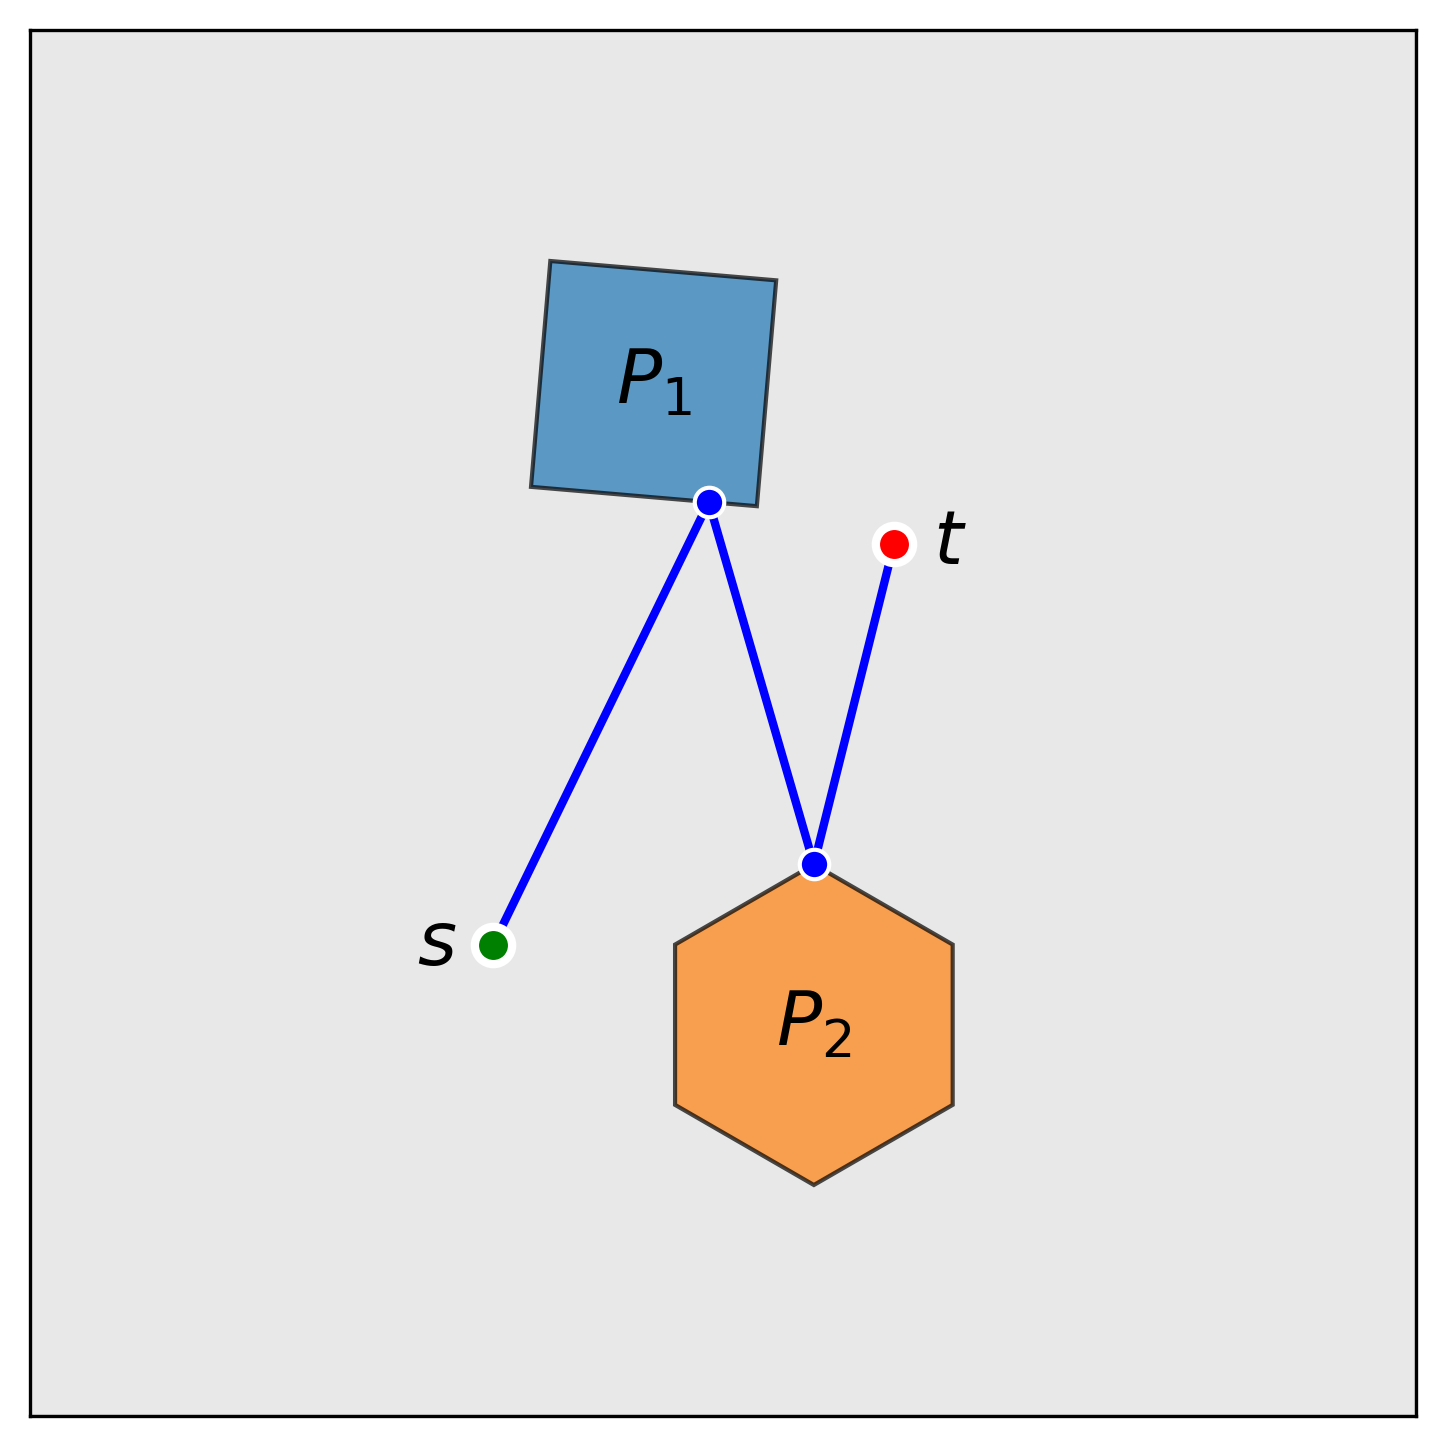
\includegraphics[width=\linewidth]{i_path.png}
	\caption{Caminho mínimo de~\(s\) até~\(t\) visitando~\(P_1\) e~\(P_2\).}
	\label{fig:i_path}
\end{minipage}
\hspace{10pt}
\begin{minipage}{0.44\textwidth}
	\centering
	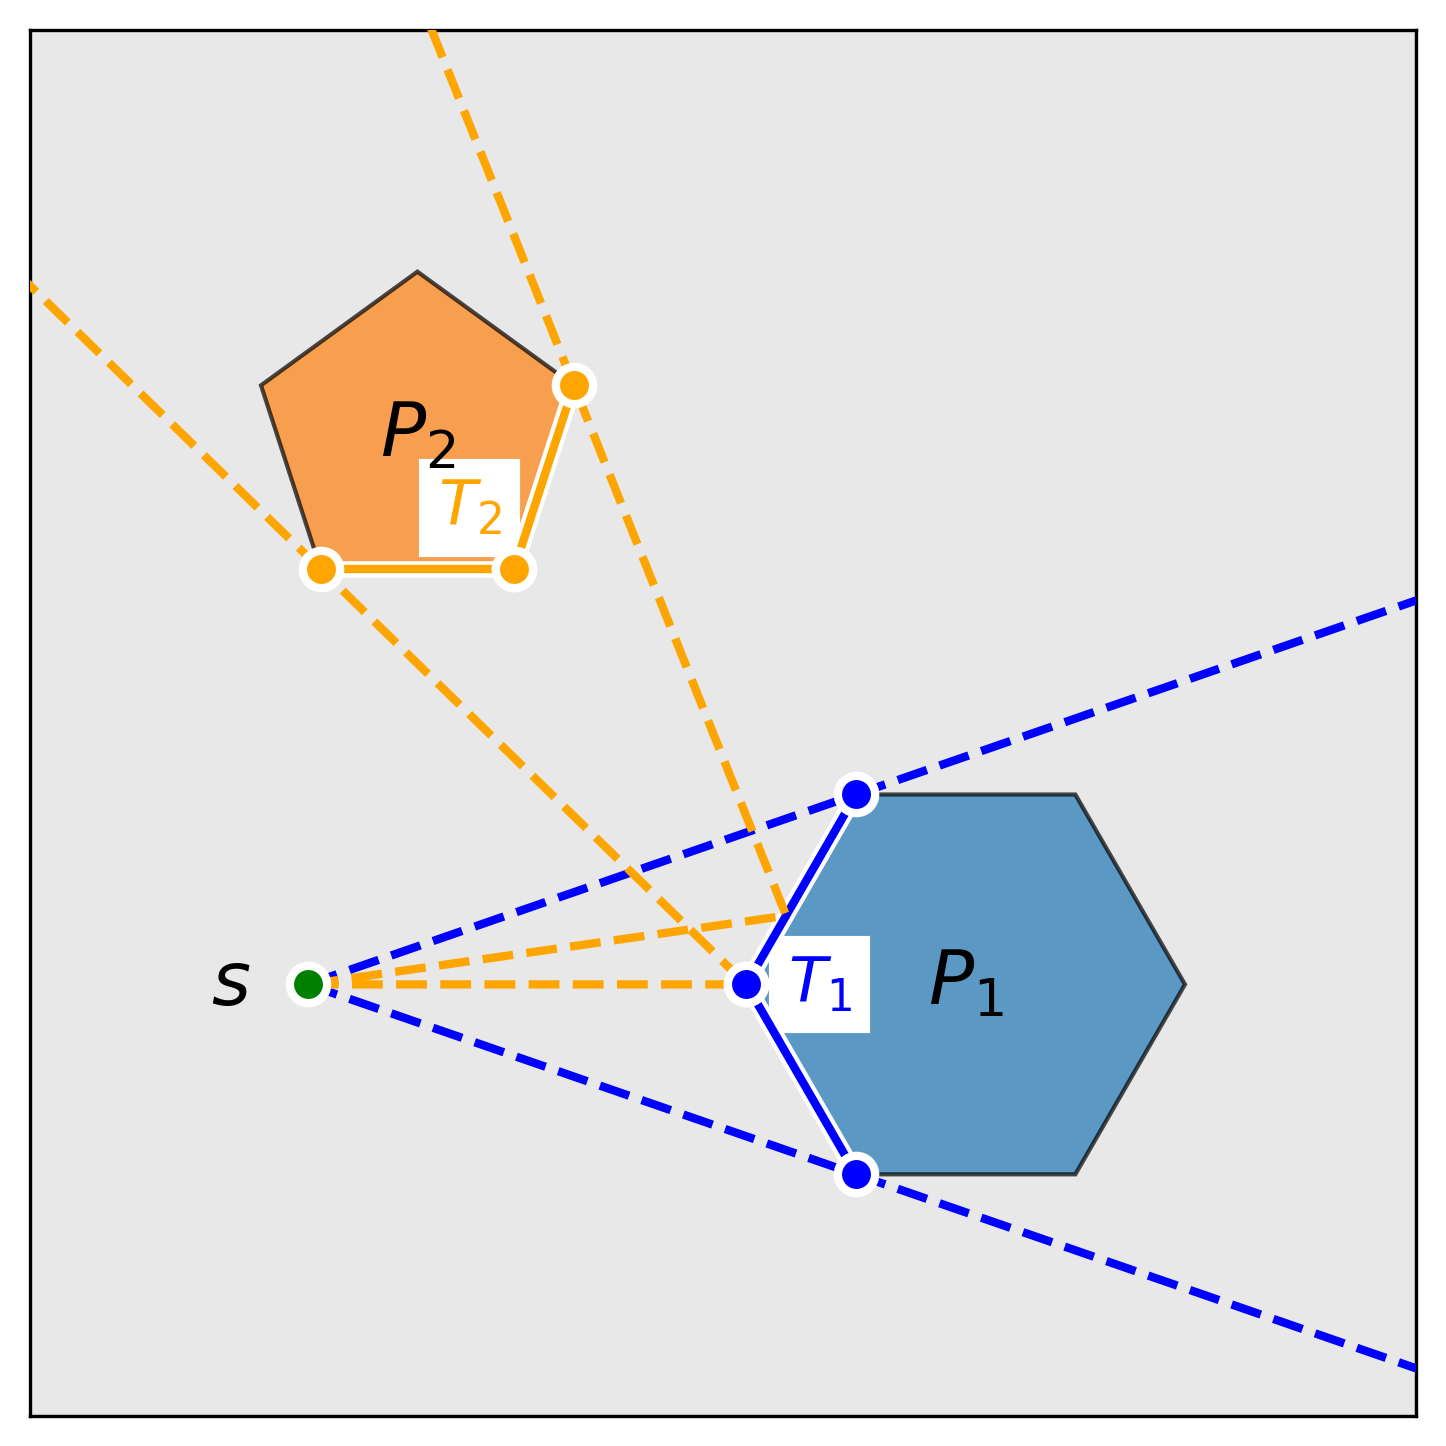
\includegraphics[width=\linewidth]{first_contact.png}
	\caption{Região de primeiro contato~\(T_1\) de~\(P_1\) e~\(T_2\) de~\(P_2\).}
	\label{fig:first_contact}
\end{minipage}
\end{figure}

\item[Mapa de Último Passo (\(S_i\)):] O mapa de último passo~\(S_i\) (\(1 \le i \le k\)) de um polígono~\(P_i\) é uma partição do plano em regiões associadas a cada vértice e a cada aresta de~\(P_i\). Um ponto~\(p \in \mathbb{R}^2\) pertence à região associada a um vértice~\(v\) se o~\(i\)-path até~\(p\) possui~\(\overline{vp}\) como último segmento; pertence à região associada a uma aresta~\(e\) se o último segmento do~\(i\)-path até~\(p\) parte do interior de~\(e\); e pertence à região de atravessar caso contrário, ou seja, quando o~\(i\)-path até~\(p\) coincide com o~\((i-1)\)-path até~\(p\). Apenas vértices e arestas em~\(T_i\) possuem regiões não degeneradas. A Figura~\ref{fig:last_step_map} apresenta um exemplo de mapa de último passo.

\begin{figure}[h!]
	\centering
	\begin{minipage}[t]{0.47\textwidth}
		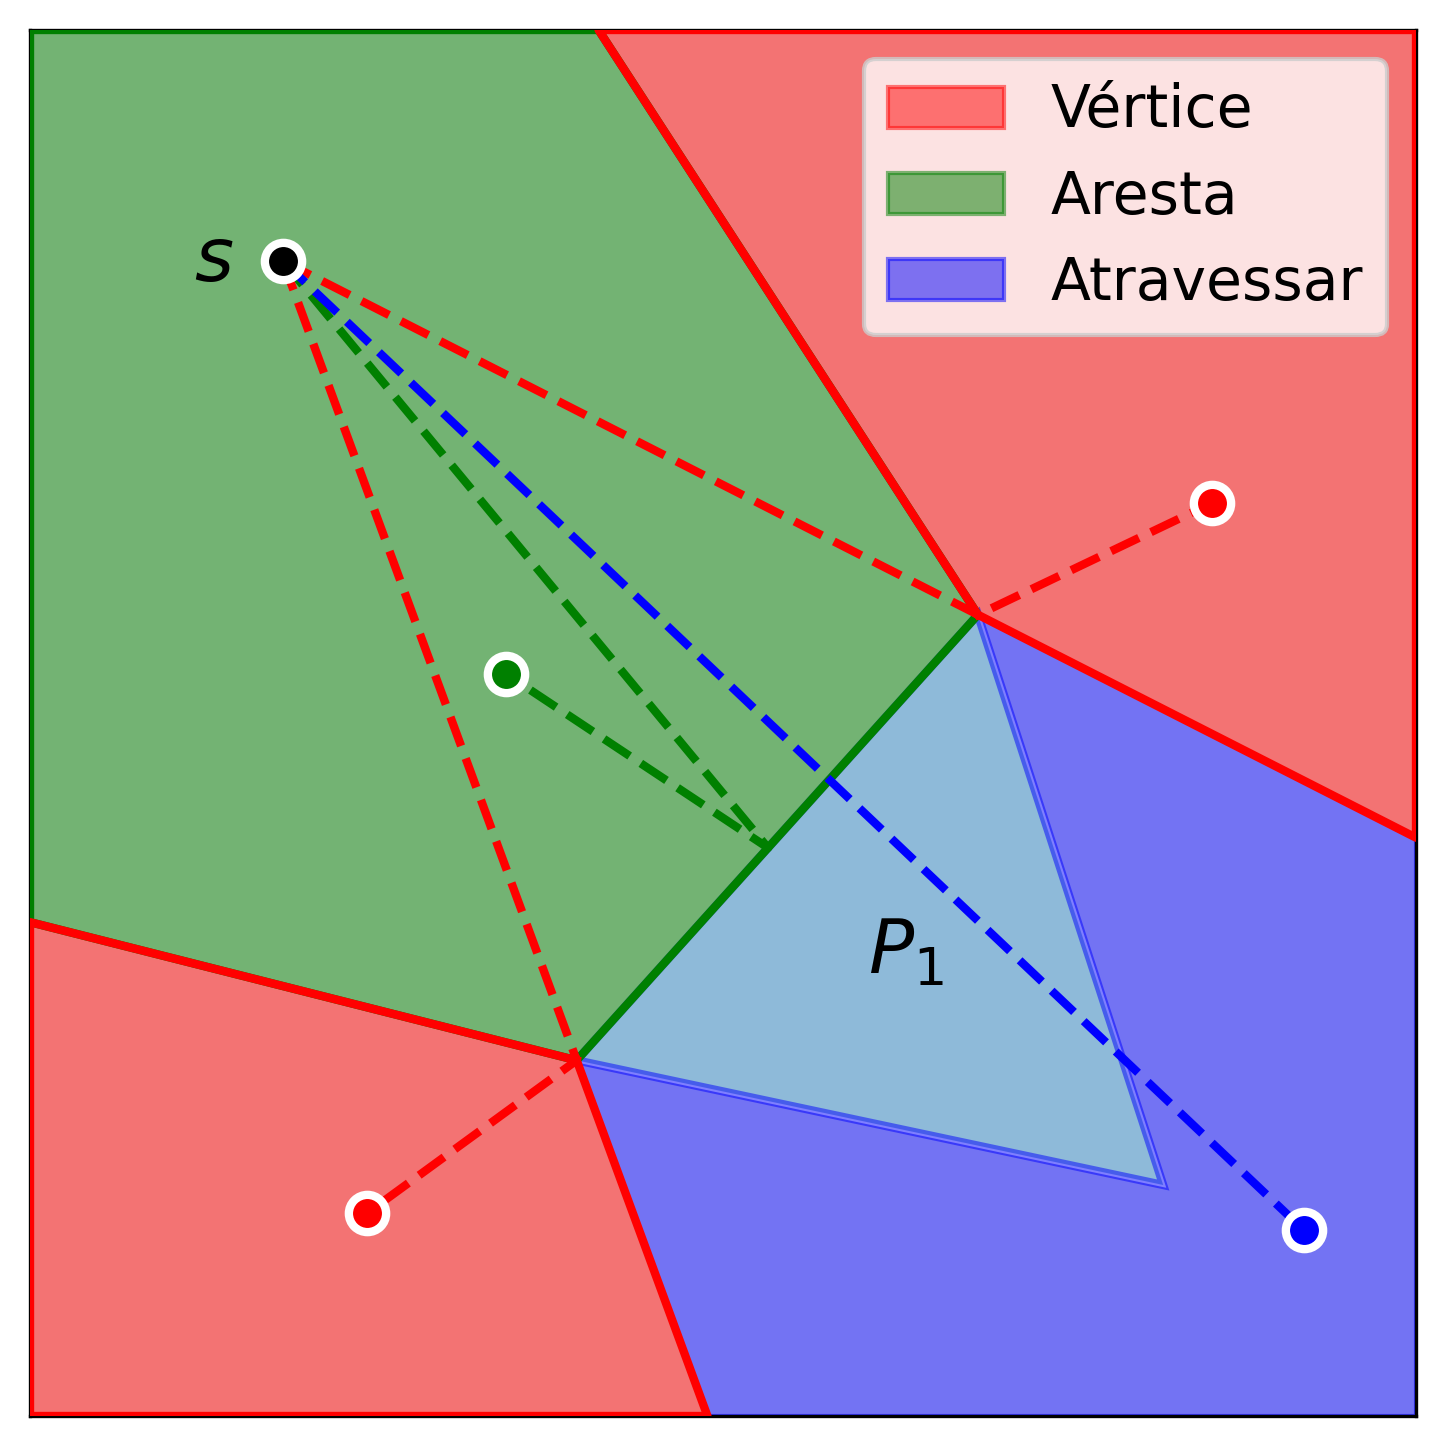
\includegraphics[width=\textwidth]{last_step_map.png}
	\end{minipage}
	\caption{Exemplo do mapa de último passo~\(S_1\) de~\(P_1\). Regiões de vértice em vermelho, de aresta em verde e de atravessar em azul, com o~\(1\)-path até um ponto representativo de cada região.}
	\label{fig:last_step_map}
\end{figure}

\end{description}

Dado um ponto~\(p \in \mathbb{R}^2\) e o mapa~\(S_i\), é possível determinar o~\(i\)-path até~\(p\) eficientemente a partir do~\((i-1)\)-path, considerando três casos:

\begin{description}

\item[Região de Vértice:] Se~\(p\) pertence à região de um vértice~\(v\), o último segmento do~\(i\)-path até~\(p\) é~\(\overline{vp}\), e o~\(i\)-path é simplesmente o~\((i-1)\)-path até~\(v\) seguido de~\(\overline{vp}\). A Figura~\ref{fig:vertex_region} ilustra essa situação com dois pontos~\(p^1\) e~\(p^2\) em regiões de vértice distintas de~\(P_2\). Note que~\(S_2\) informa apenas o último segmento do caminho, não o caminho completo: o último segmento até~\(q^1\) parte de um vértice de~\(P_1\), enquanto o até~\(q^2\) parte do interior de uma aresta de~\(P_1\), o que só se descobre consultando~\(S_1\).

\item[Região de Atravessar:] Se~\(p\) pertence à região de atravessar, o~\(i\)-path até~\(p\) coincide com o~\((i-1)\)-path até~\(p\), pois o caminho ótimo simplesmente atravessa~\(P_i\) sem desviar. A Figura~\ref{fig:pass_through} ilustra esse caso.

\begin{figure}[h!]
\centering
\begin{minipage}{0.44\textwidth}
	\centering
	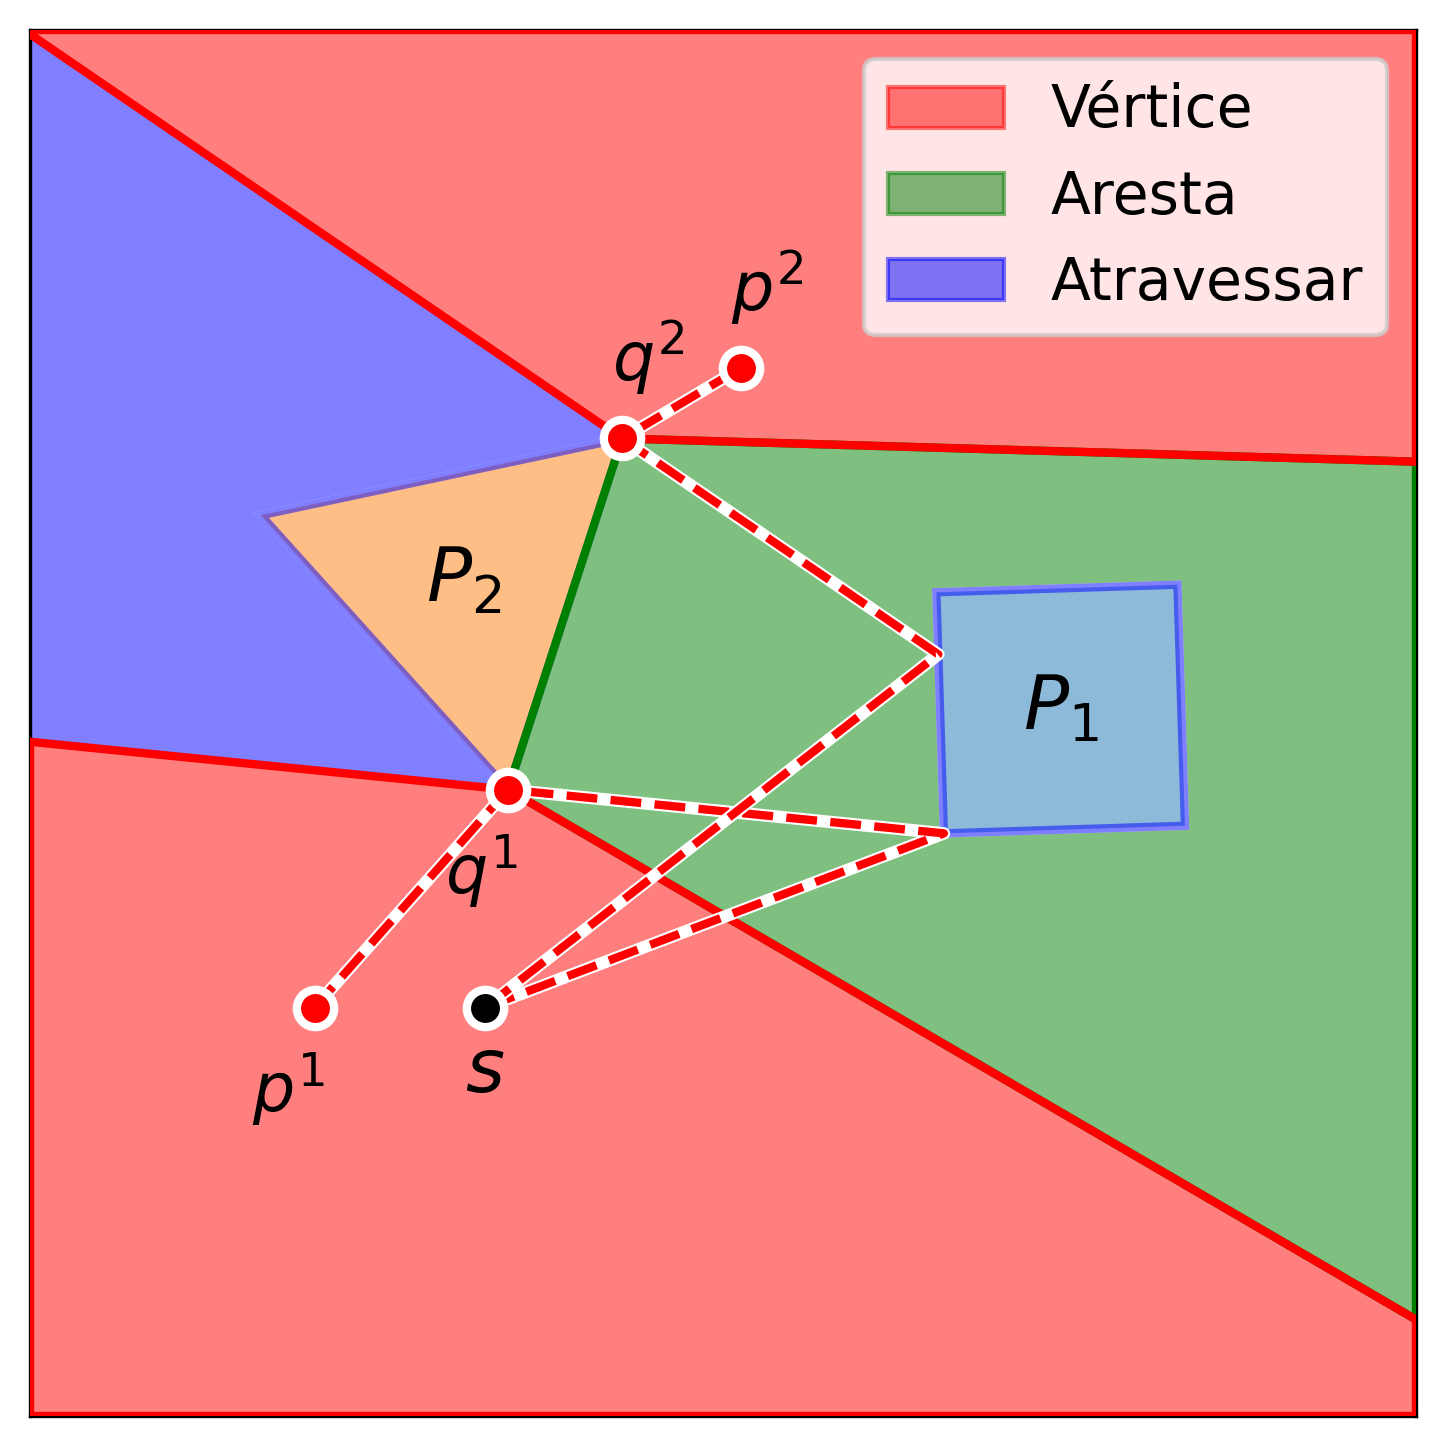
\includegraphics[width=\linewidth]{paths-vertices.png}
	\caption{\(2\)-path até~\(p^1\) e~\(p^2\), em regiões de vértice de~\(P_2\).}
	\label{fig:vertex_region}
\end{minipage}
\hspace{10pt}
\begin{minipage}{0.44\textwidth}
	\centering
	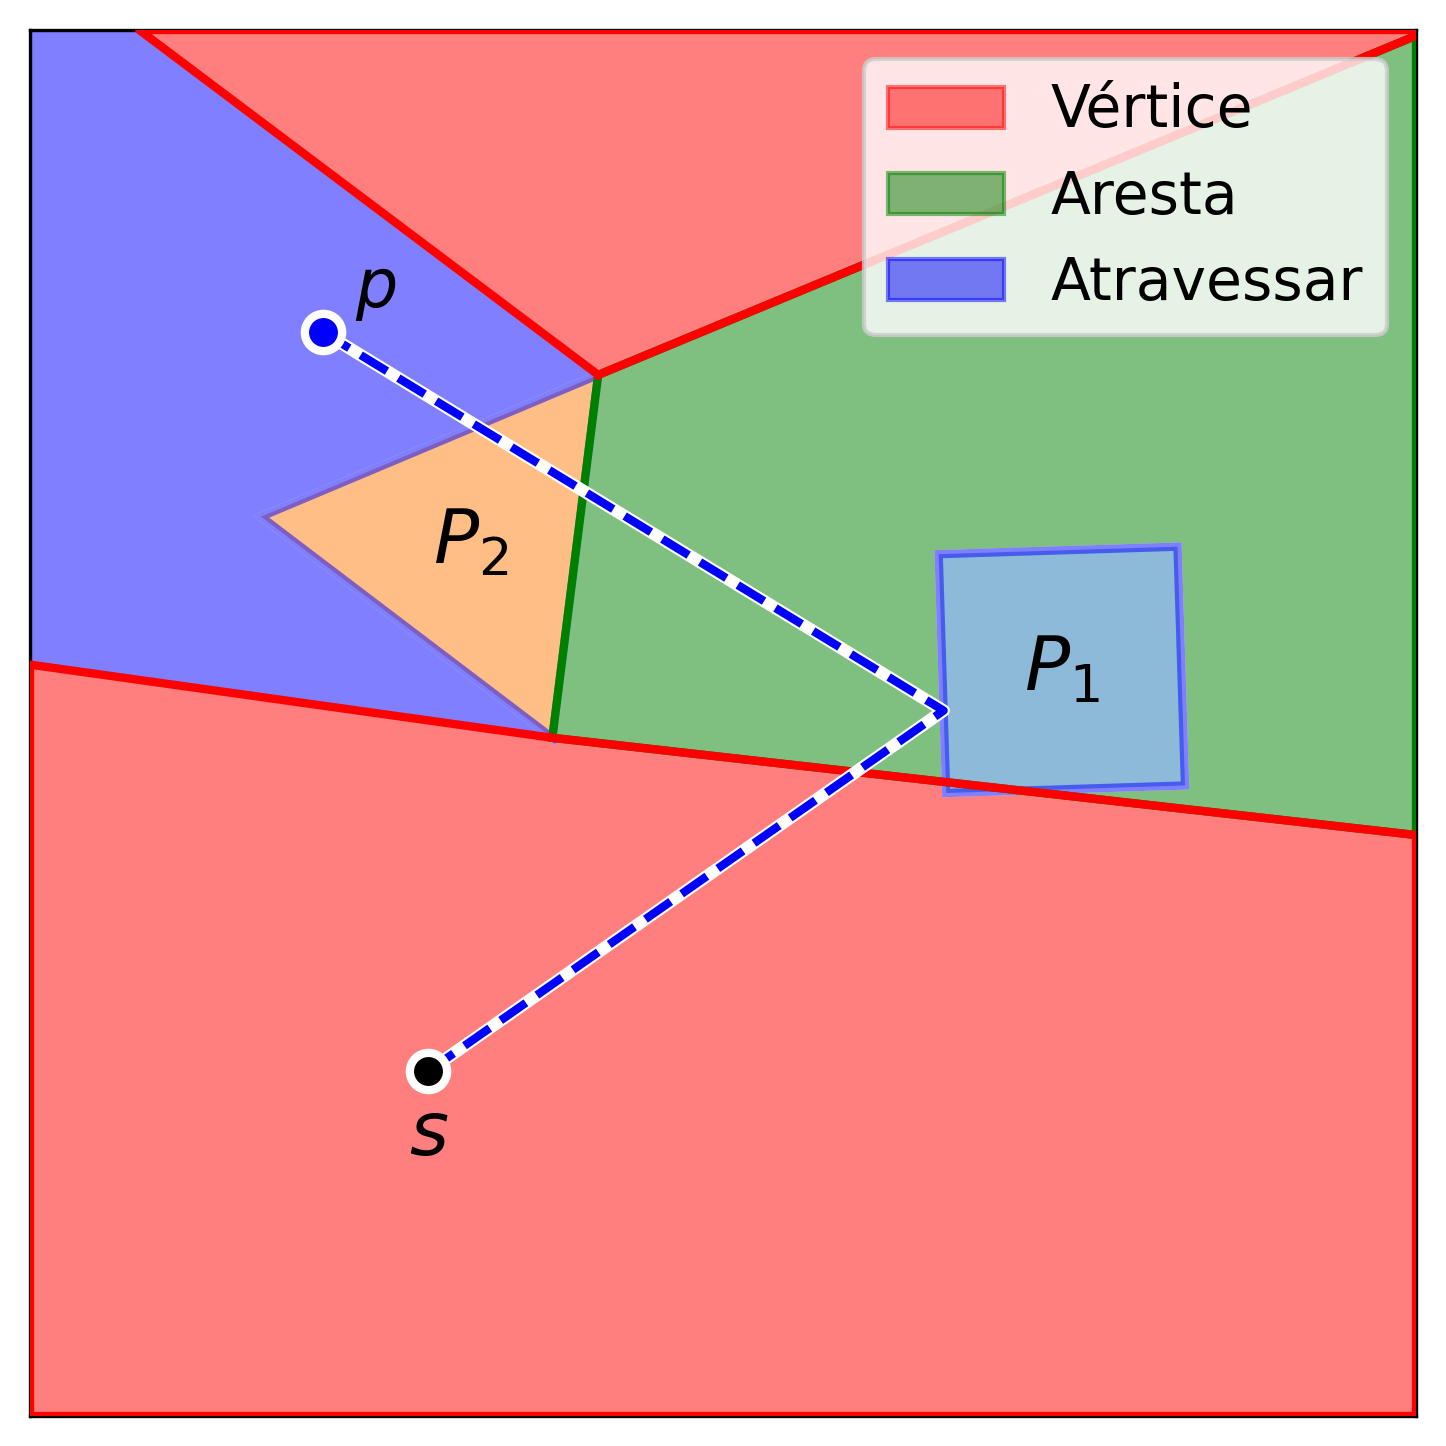
\includegraphics[width=\linewidth]{paths-pass.png}
	\caption{\(2\)-path até~\(p\), em região de atravessar de~\(P_2\).}
	\label{fig:pass_through}
\end{minipage}
\end{figure}

\item[Região de Aresta:] Se~\(p\) pertence à região de uma aresta~\(e = \overline{uv}\), reflete-se~\(p\) em relação à reta que contém~\(e\), obtendo~\(p'\). O~\(i\)-path até~\(p\) é então a parte do~\((i-1)\)-path até~\(p'\) desde~\(s\) até o ponto~\(q\) de interseção do último segmento desse caminho com~\(e\), seguida de~\(\overline{qp}\). A Figura~\ref{fig:edge_region} ilustra essa construção. As fórmulas para~\(p'\) e~\(q\) são:
\begin{align}
	p' &= -p + 2u + 2\frac{(p - u) \cdot (v - u)}{\|v - u\|^2}(v - u), \label{eq:reflection_on_edge} \\
	q  &= q' + \frac{(u - q') \times (v - u)}{(p' - q') \times (v - u)}(p' - q'). \label{eq:intersection_on_edge}
\end{align}

\begin{figure}[h!]
\centering
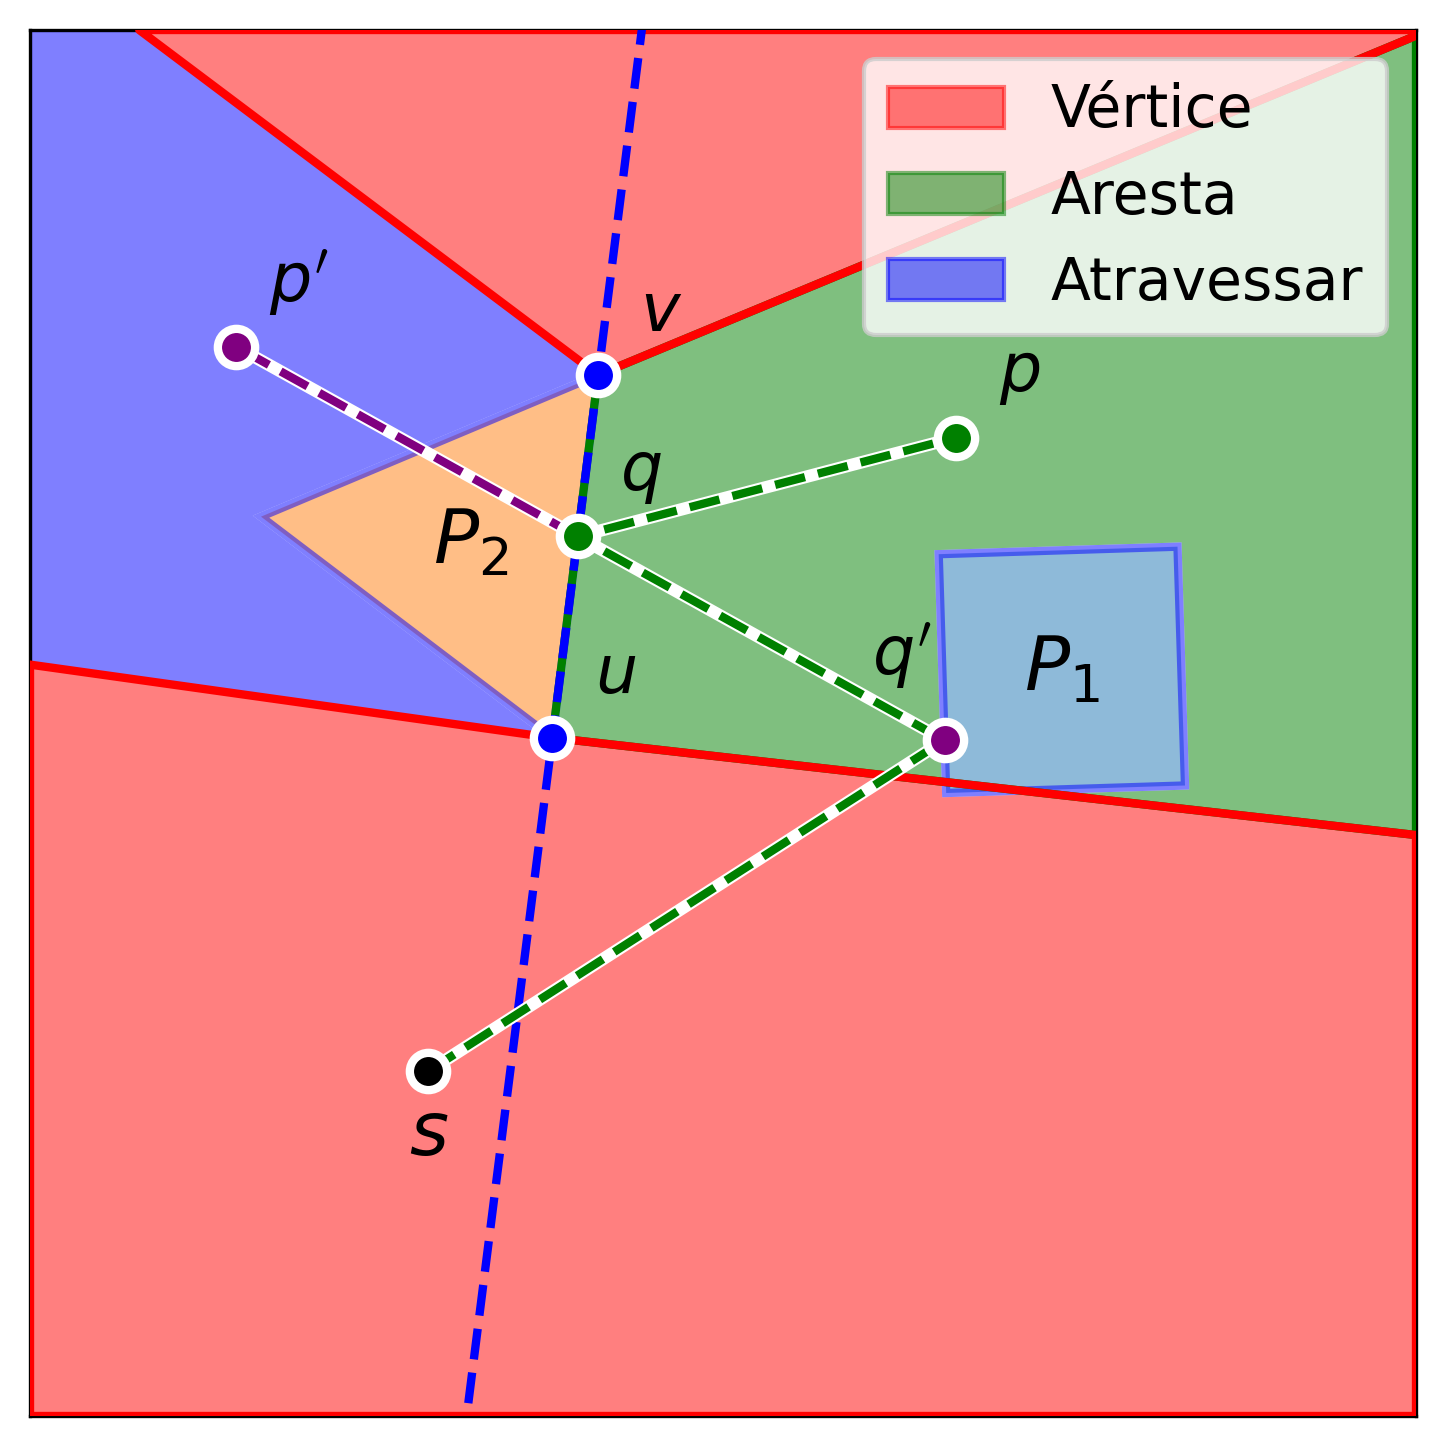
\includegraphics[width=0.5\linewidth]{paths-edge.png}
\caption{\(2\)-path até~\(p\), em região de aresta de~\(P_2\). O ponto~\(p'\) é a reflexão de~\(p\), \(q'\) precede~\(p'\) no~\(1\)-path, e~\(q\) é a interseção de~\(\overline{q'p'}\) com~\(e\).}
\label{fig:edge_region}
\end{figure}

\end{description}

\subsection{O Algoritmo}

O algoritmo opera em duas fases. Na primeira, para cada~\(i = 1, \dots, k\), calcula-se~\(T_i\) e em seguida~\(S_i\), usando os mapas já computados. Na segunda, consulta-se o~\(k\)-path até~\(t\). A seguir, detalha-se cada etapa.

\subsubsection{Região de Primeiro Contato}

Para determinar~\(T_i\), basta verificar cada aresta de~\(P_i\): uma aresta~\(e = \overline{uv}\) pertence a~\(T_i\) se e somente se~\((v - u) \times (q - u) < 0\), onde~\(q\) é o ponto que precede~\(u\) no~\((i-1)\)-path até~\(u\). Essa verificação é implementada no Algoritmo~\algref{alg:first_contact_region}. Os algoritmos a seguir fazem uso de uma função auxiliar \texttt{ConsultaÚltimoPasso}\((p, i, \dots)\), que dado um ponto~\(p \in \mathbb{R}^2\) e um índice~\(i\), retorna o ponto que precede~\(p\) no~\(i\)-path até~\(p\); essa função será implementada na Seção~\ref{sec:query}, após a definição de \texttt{LocalizaPonto}.

\begin{algorithm}[h!]
\alglabel{alg:first_contact_region}
\caption{Região de Primeiro Contato}
\Input{\(i, s, (P_1, \dots, P_i), (T_1, \dots, T_{i-1}), (S_1, \dots, S_{i-1})\)}
\Output{Região de primeiro contato~\(T_i\) de~\(P_i\) como conjunto de arestas.}
\vspace{0.3em}\hrule\vspace{0.3em}
\Function{RegiãoDePrimeiroContato\((i, s, \dots)\)}{
	\(T_i \leftarrow \emptyset\) \\
	\For{cada aresta~\(e = \overline{uv}\) de~\(P_i\)}{
		\(q \leftarrow \text{ConsultaÚltimoPasso}(u, i-1, \dots)\) \\
		\If{\((v - u) \times (q - u) < 0\)}{
			\(T_i \leftarrow T_i \cup \{e\}\)
		}
	}
	\Return{}~\(T_i\)
}
\end{algorithm}

\subsubsection{Mapa de Último Passo}

Para calcular~\(S_i\), utilizam-se as condições de otimalidade local de~\cite{tpp-dror-2003}. Para cada vértice~\(v\) de~\(P_i\) com arestas incidentes~\(e^1\) e~\(e^2\), calcula-se um par de raios~\((r^1, r^2)\) que delimita a região de vértice associada a~\(v\) em~\(S_i\), conforme o Lema~\ref{lemma:last_step}.

\begin{blockQuote}
\begin{lemma}
Seja~\(v\) um vértice de~\(P_i\) com arestas incidentes~\(e^1\) e~\(e^2\), e seja~\(q\) o ponto que precede~\(v\) no~\((i-1)\)-path até~\(v\). O raio associado a uma aresta~\(e\) incidente a~\(v\) é~\(v - q\) se~\(q\) está do lado interno de~\(e\), ou~\(r_\perp(q, v, e)\) caso contrário, onde~\(r_\perp(q, v, e)\) denota a reflexão do vetor~\(q - v\) em relação à reta perpendicular a~\(e\) que passa por~\(v\). O par ordenado~\((r^1, r^2)\) assim obtido delimita exatamente a região de vértice de~\(v\) em~\(S_i\). \label{lemma:last_step}
\end{lemma}
\end{blockQuote}

A reflexão~\(r_\perp(q, v, e)\) de~\(q - v\) em relação à perpendicular a~\(e = \overline{uv}\) em~\(v\) é dada por:
\[
	r_\perp(q, v, e) = (q - v) - 2\frac{(q - v) \cdot \hat{e}}{\|\hat{e}\|^2}\hat{e}, \quad \hat{e} = v - u,
\]
onde~\(\cdot\) denota o produto interno em~\(\mathbb{R}^2\). Esse cálculo é implementado no Algoritmo~\algref{alg:last_step_map}.

\begin{algorithm}[h!]
\alglabel{alg:last_step_map}
\caption{Mapa de Último Passo}
\Input{\(i, s, (P_1, \dots, P_i), (T_1, \dots, T_i), (S_1, \dots, S_{i-1})\)}
\Output{Mapa de último passo~\(S_i\) como associação de pares de raios aos vértices de~\(P_i\).}
\vspace{0.3em}\hrule\vspace{0.3em}
\Function{Reflexão\((q, v, e)\)}{
	\If{\(e \in T_i\)}{
		\Return{} reflexão de~\(q - v\) em relação à perpendicular a~\(e\) em~\(v\)
	}
	\Else{
		\Return{}~\(v - q\)
	}
}
\Function{MapaDeÚltimoPasso\((i, s, \dots)\)}{
	\(S_i \leftarrow \emptyset\) \\
	\For{cada vértice~\(v\) de~\(P_i\) com arestas incidentes~\(e^1\) e~\(e^2\)}{
		\(q \leftarrow \text{ConsultaÚltimoPasso}(v, i-1, \dots)\) \\
		\(r^1 \leftarrow \text{Reflexão}(q, v, e^1)\) \\
		\(r^2 \leftarrow \text{Reflexão}(q, v, e^2)\) \\
		Associa~\((r^1, r^2)\) a~\(v\) em~\(S_i\)
	}
	\Return{}~\(S_i\)
}
\end{algorithm}

\subsubsection{Localização de Pontos e Busca Binária}

Com~\(S_i\) calculado, o passo central é localizar um ponto~\(p \in \mathbb{R}^2\) no mapa~\(S_i\). Descreve-se a seguir como realizar cada verificação em tempo~\(O(1)\).
\paragraph{Região de vértice.} Seja~\(v\) um vértice com raios associados~\((r^1, r^2)\) em~\(S_i\). O ponto~\(p\) pertence à região de~\(v\) se está no cone definido por~\(v\) e pelos raios~\(r^1\) e~\(r^2\) em sentido anti-horário. Se o ângulo de abertura é inferior a~\(180^\circ\) (\(r^1 \times r^2 \ge 0\)), exige-se~\(r^1 \times (p - v) > 0\) e~\(r^2 \times (p - v) < 0\); caso contrário (\(r^1 \times r^2 < 0\)), basta uma das duas condições.

\paragraph{Região de aresta.} Seja~\(e = \overline{uv}\) uma aresta de~\(T_i\), com~\(r^1\) o segundo raio de~\(u\) e~\(r^2\) o primeiro raio de~\(v\) em~\(S_i\). O ponto~\(p\) pertence à região de~\(e\) se e somente se:
\[
	r^1 \times (p - u) > 0 \quad \text{e} \quad r^2 \times (p - v) < 0 \quad \text{e} \quad (v - u) \times (p - u) < 0.
\]

\paragraph{Busca binária via arestas fictícias.} Uma abordagem direta para localizar~\(p\) em~\(S_i\) verificaria cada região de vértice e aresta de~\(T_i\) sequencialmente, com custo~\(O(|T_i|)\). Para melhorar isso, observa-se que as verificações acima se generalizam naturalmente para subconjuntos contíguos de vértices. Dado um subconjunto~\(v^l, \dots, v^r\) de vértices consecutivos de~\(P_i\), define-se uma \textit{aresta fictícia} entre~\(v^l\) e~\(v^r\) usando os primeiros raios de~\(v^l\) e~\(v^r\) em~\(S_i\). A região associada a essa aresta fictícia contempla exatamente as regiões de vértice de~\(v^l\) até~\(v^{r-1}\) e as regiões de aresta entre eles, totalizando~\(r - l\) regiões de cada tipo. Formalmente, um ponto~\(p\) pertence à região da aresta fictícia se e somente se pertence a alguma dessas regiões, ou a parte do interior de~\(P_i\) delimitada por~\(v^l\) e~\(v^r\). Como os polígonos são disjuntos,~\(p\) nunca está no interior de~\(P_i\), de modo que essa ambiguidade não afeta a corretude do algoritmo. A verificação pode ser feita em tempo~\(O(1)\), considerando quatro casos dependendo de se os raios~\(r^1\) e~\(r^2\) estão do lado interno ou externo da aresta fictícia. A Figura~\ref{fig:fake_edge} ilustra a construção e a Figura~\ref{fig:binary_search_cases} os quatro casos.

\begin{figure}[h!]
	\centering
	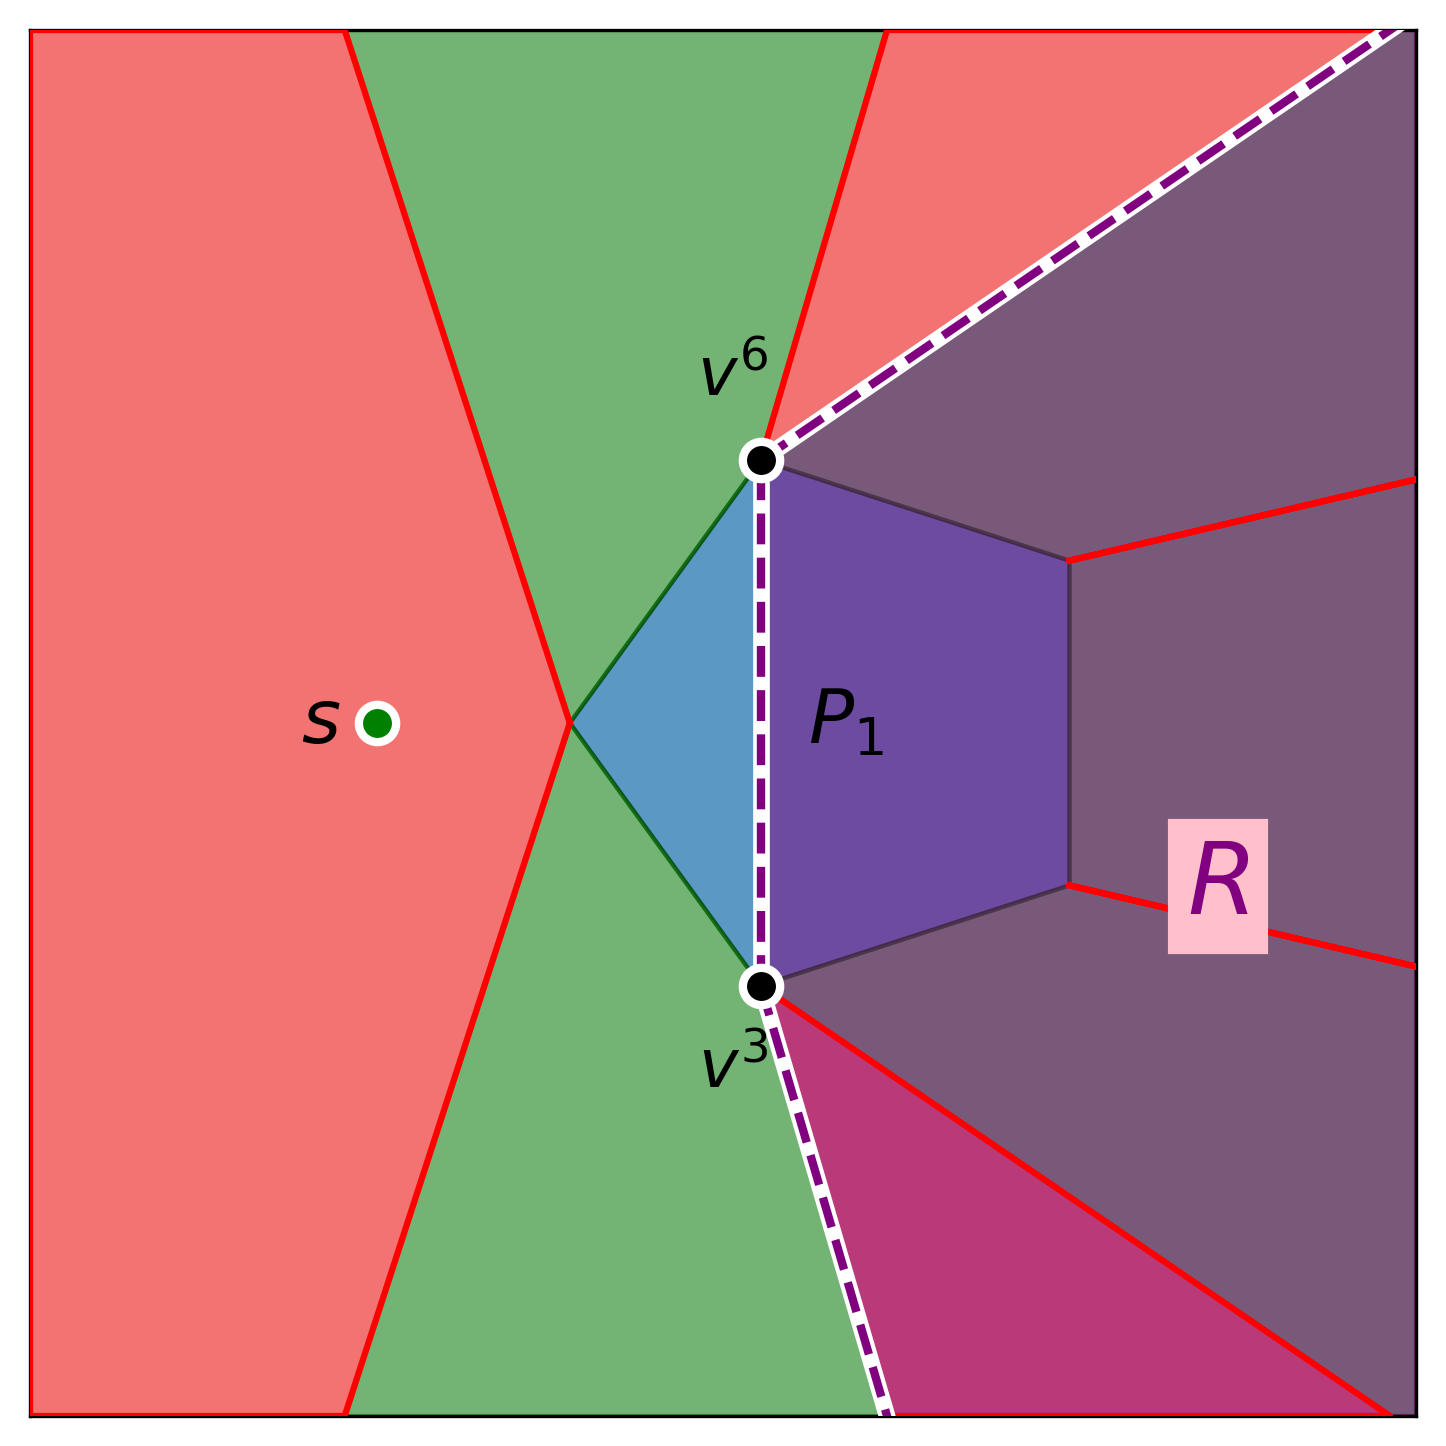
\includegraphics[width=0.45\linewidth]{fake_edge.png}
	\caption{Aresta fictícia entre~\(v^3\) e~\(v^6\) de~\(P_1\), cobrindo as regiões de vértice de~\(v^3, v^4, v^5\) e das arestas entre eles.}
	\label{fig:fake_edge}
\end{figure}

\begin{figure}[h!]
	\centering
	\begin{subfigure}[b]{0.37\textwidth}
		\centering
		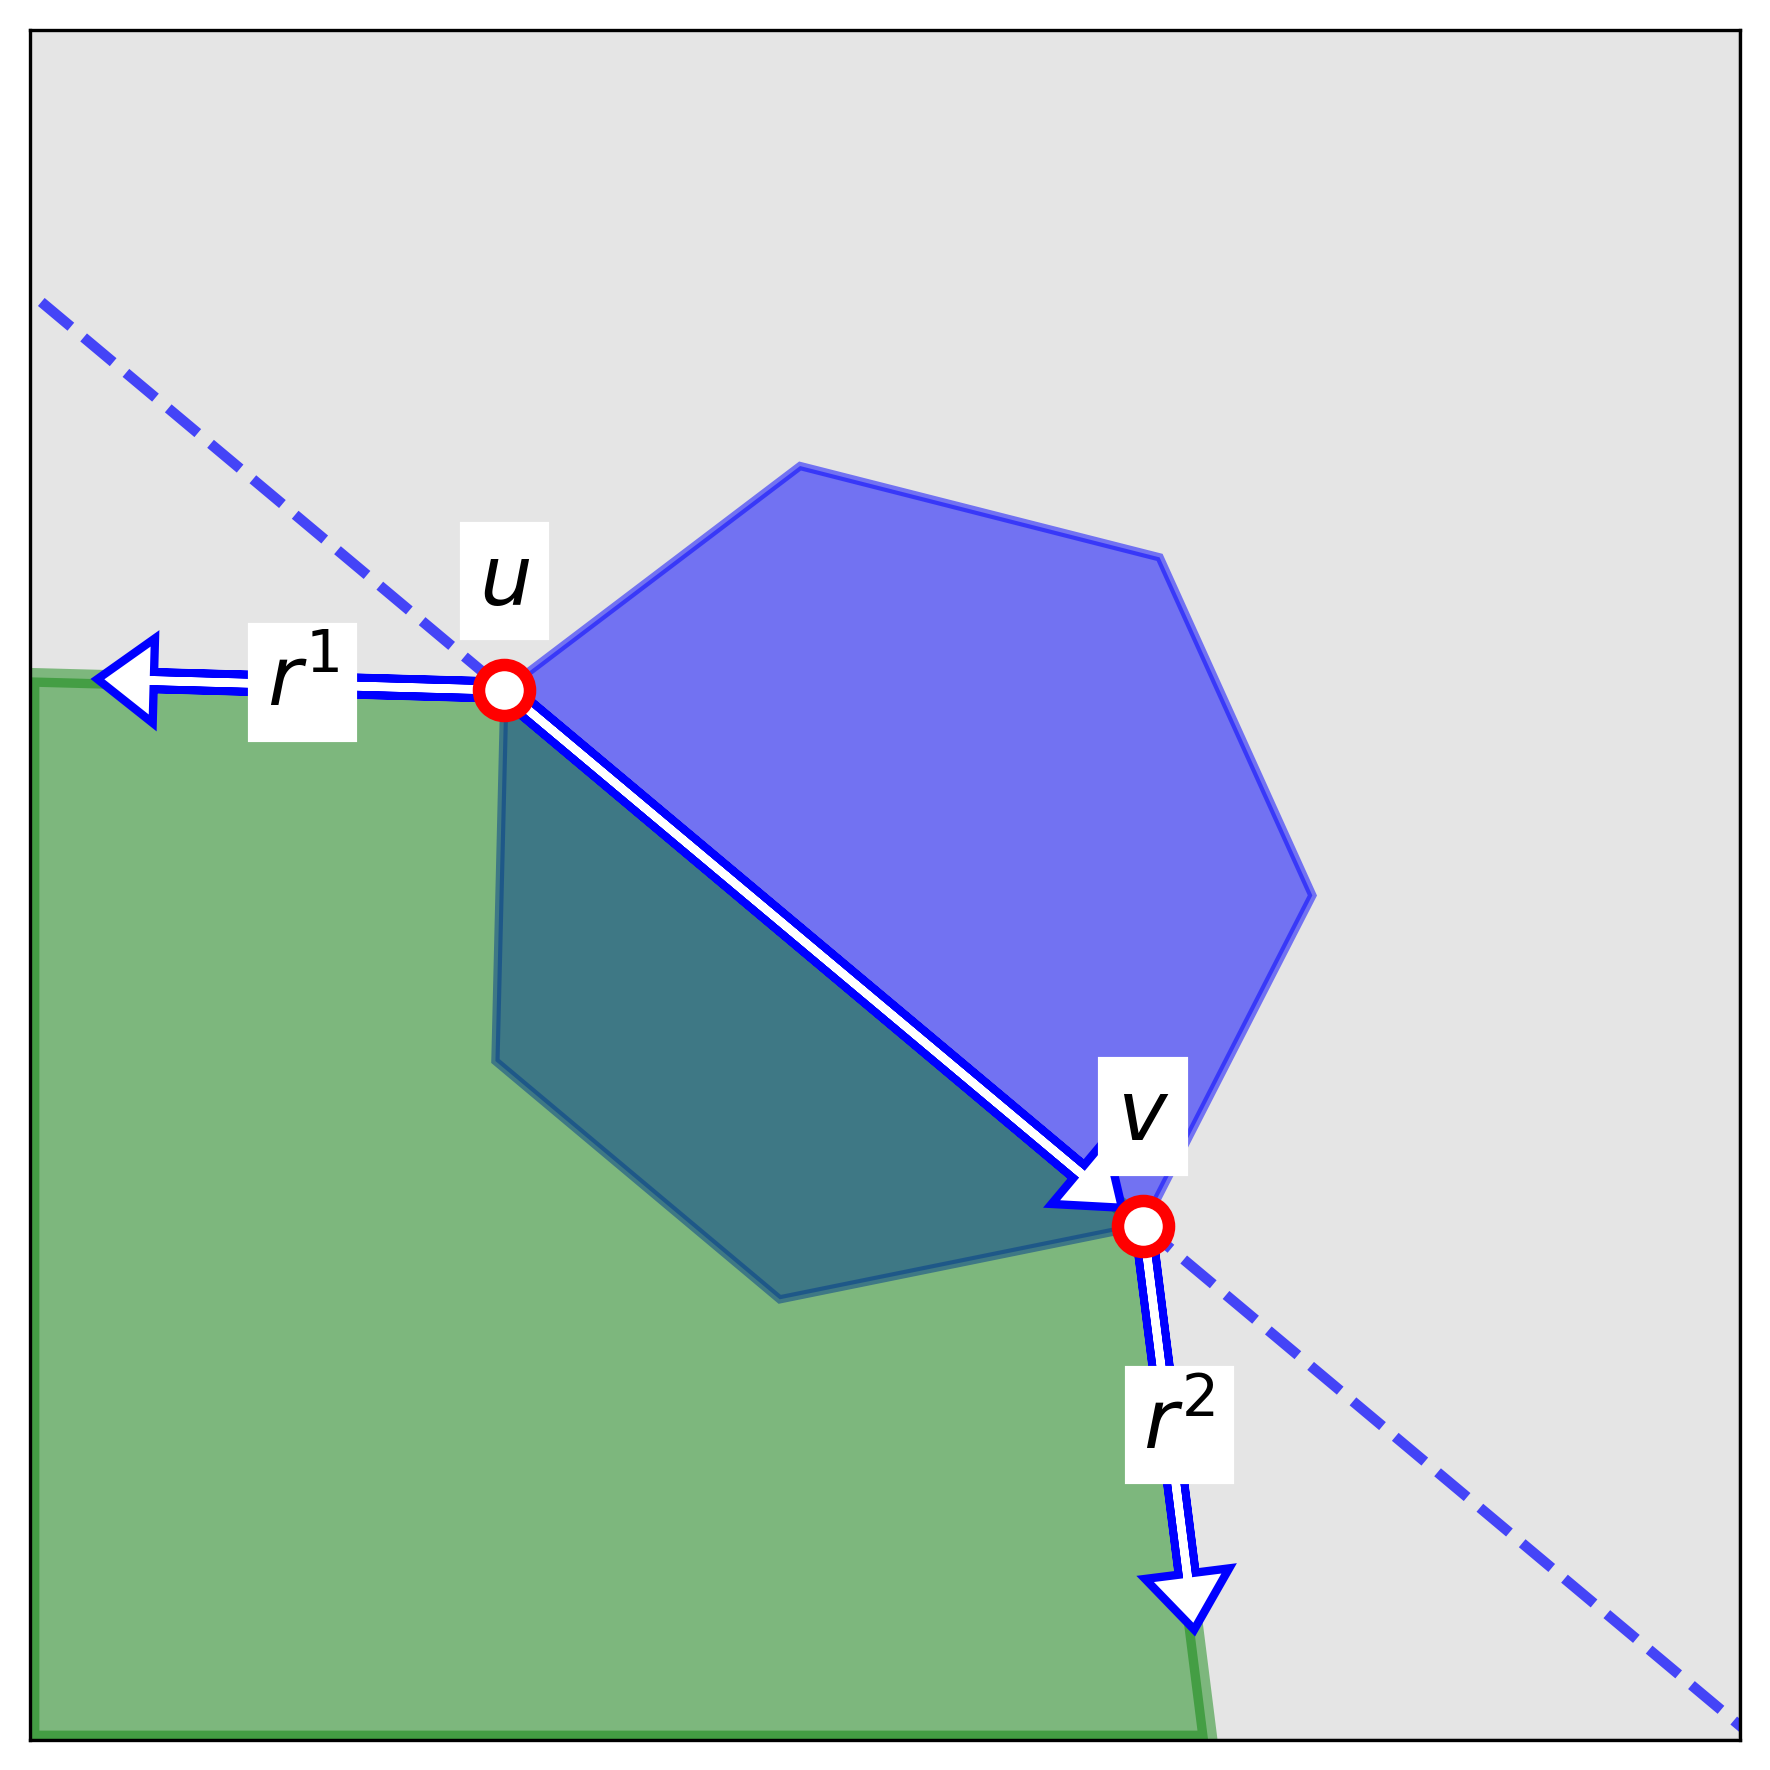
\includegraphics[width=\textwidth]{binary_search_cases-1.png}
		\caption{\(r^1\) e~\(r^2\) externos.}
	\end{subfigure}
	\hspace{0.5cm}
	\begin{subfigure}[b]{0.37\textwidth}
		\centering
		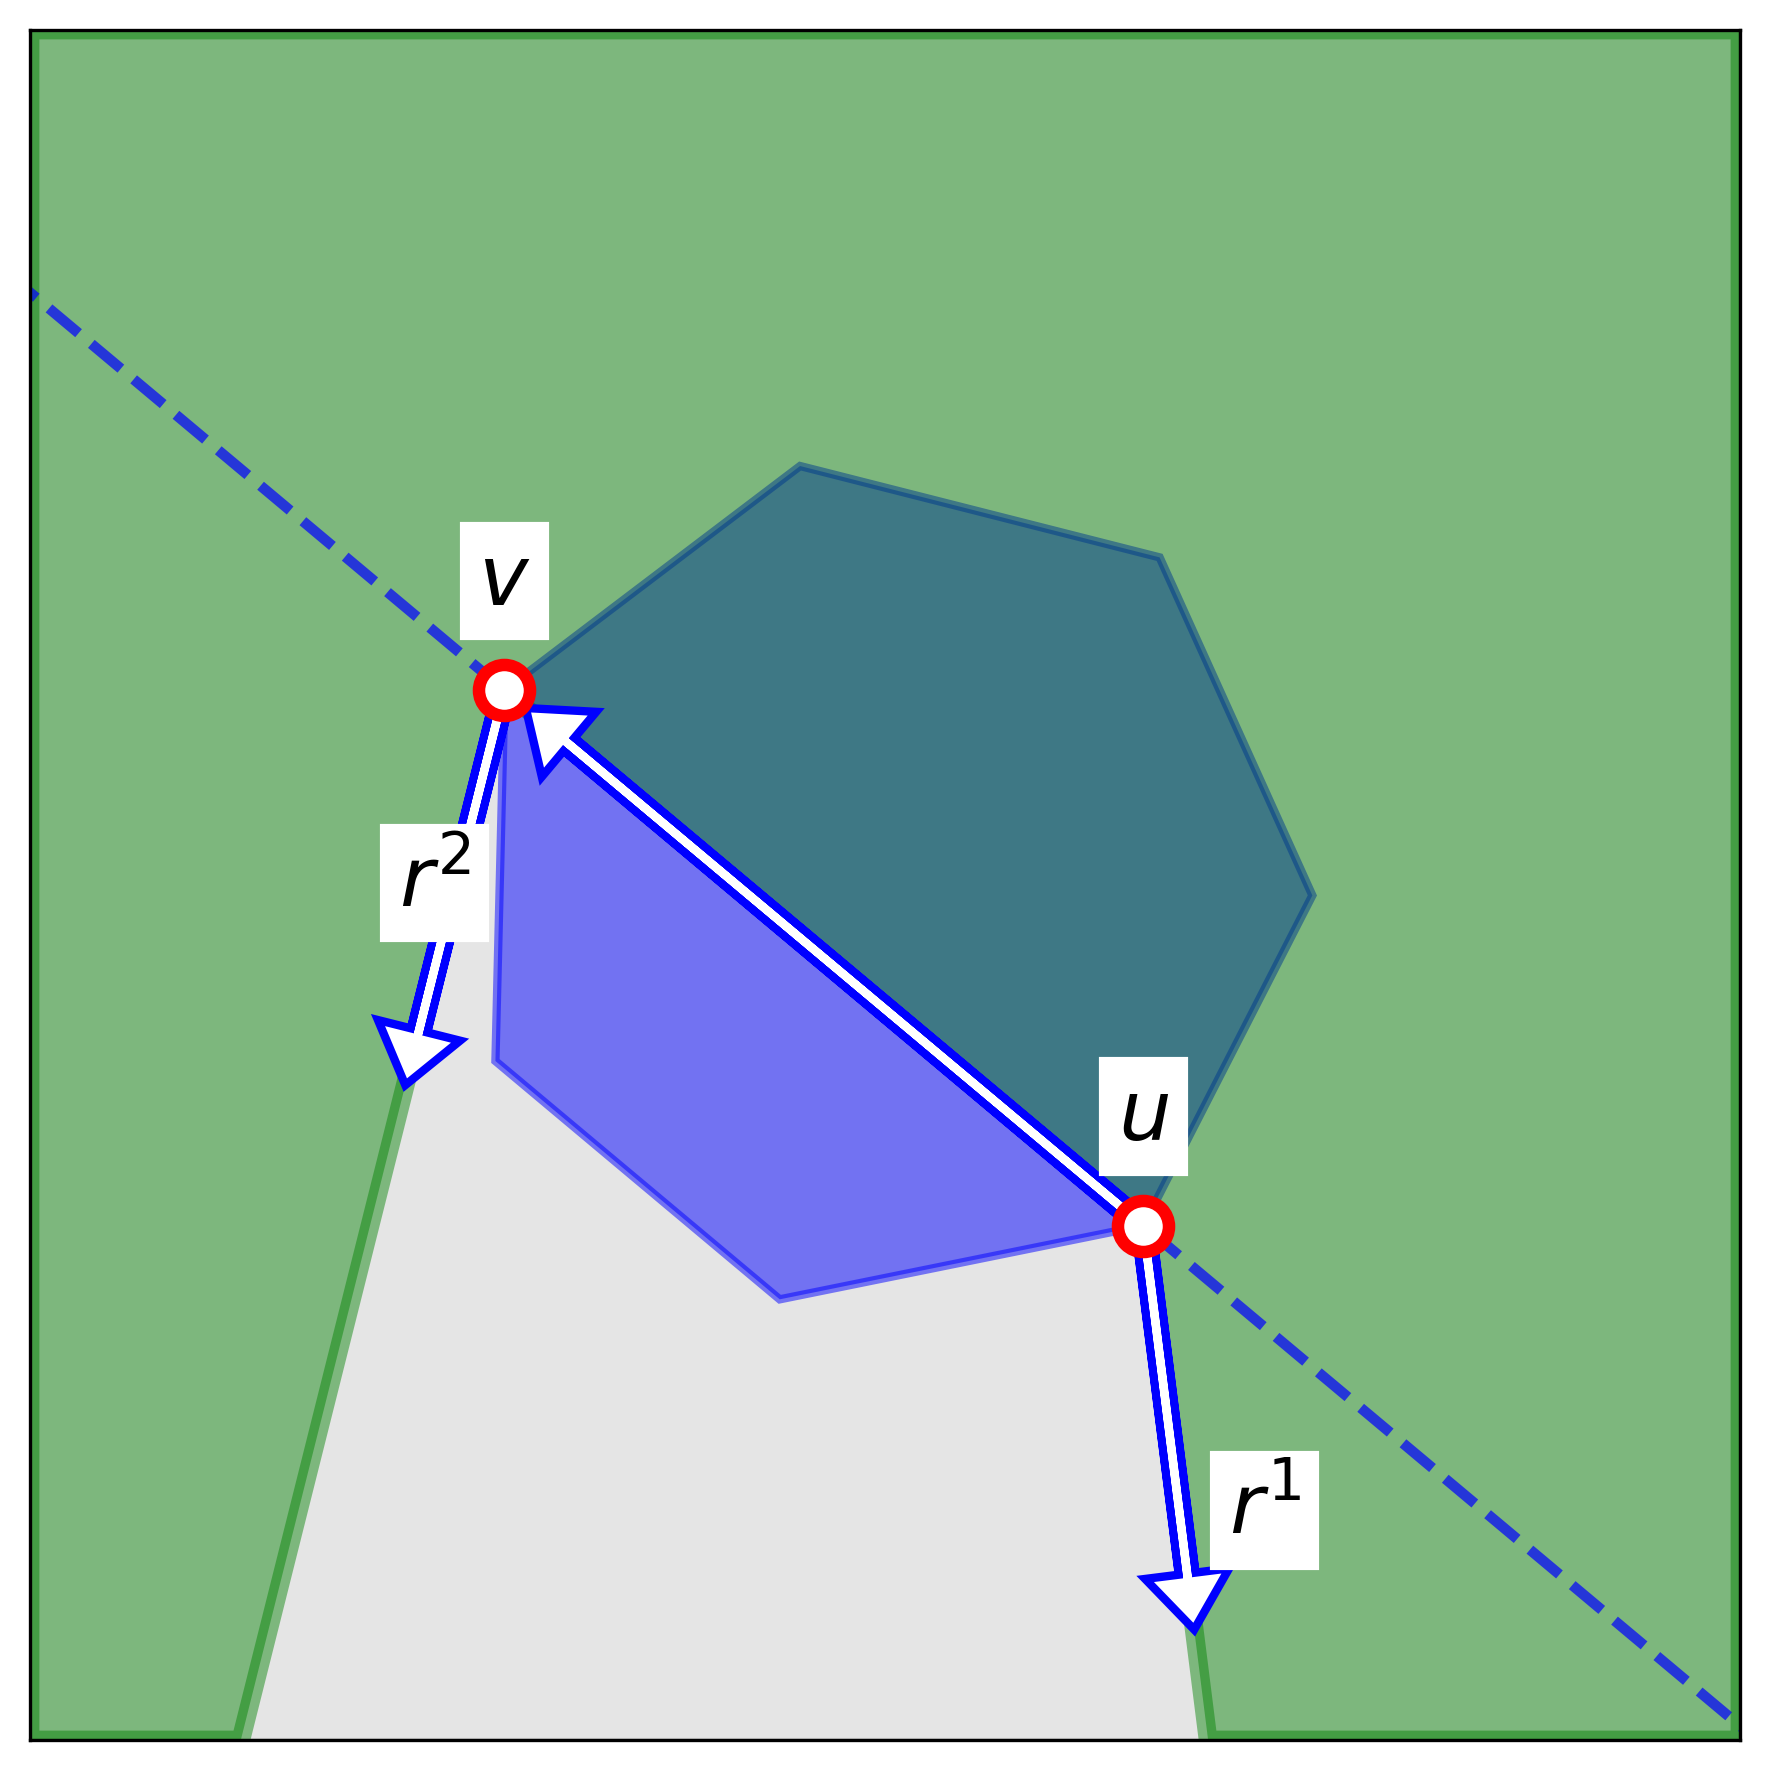
\includegraphics[width=\textwidth]{binary_search_cases-2.png}
		\caption{\(r^1\) e~\(r^2\) internos.}
	\end{subfigure}
	\medskip
	\begin{subfigure}[b]{0.37\textwidth}
		\centering
		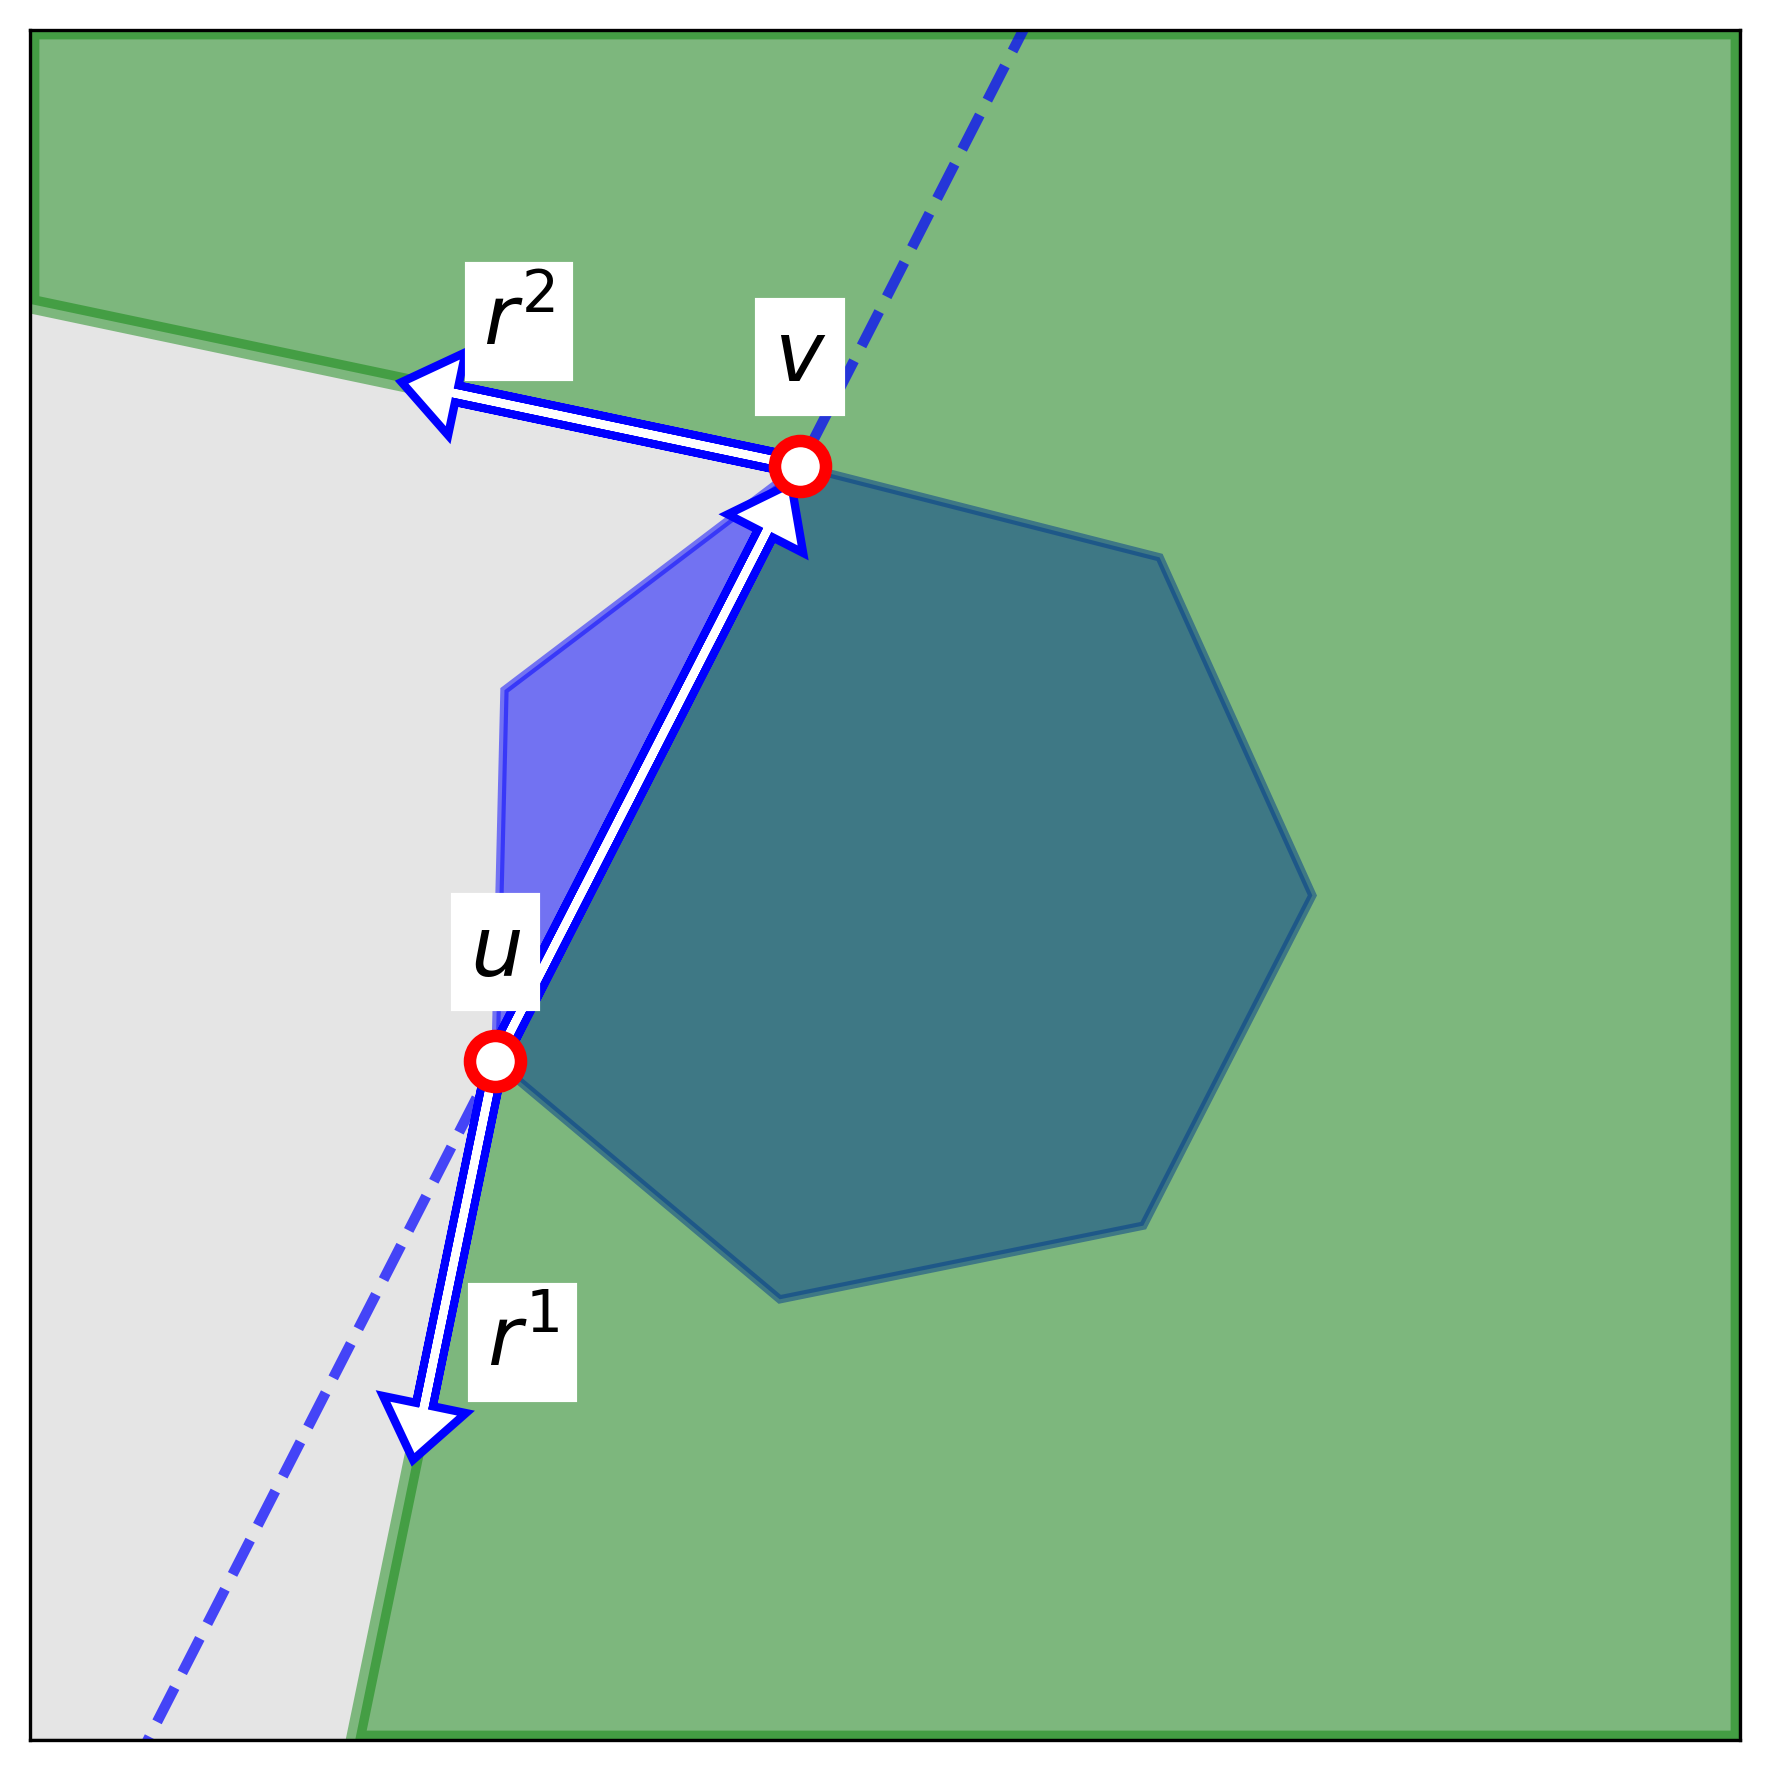
\includegraphics[width=\textwidth]{binary_search_cases-3.png}
		\caption{\(r^1\) externo,~\(r^2\) interno.}
	\end{subfigure}
	\hspace{0.5cm}
	\begin{subfigure}[b]{0.37\textwidth}
		\centering
		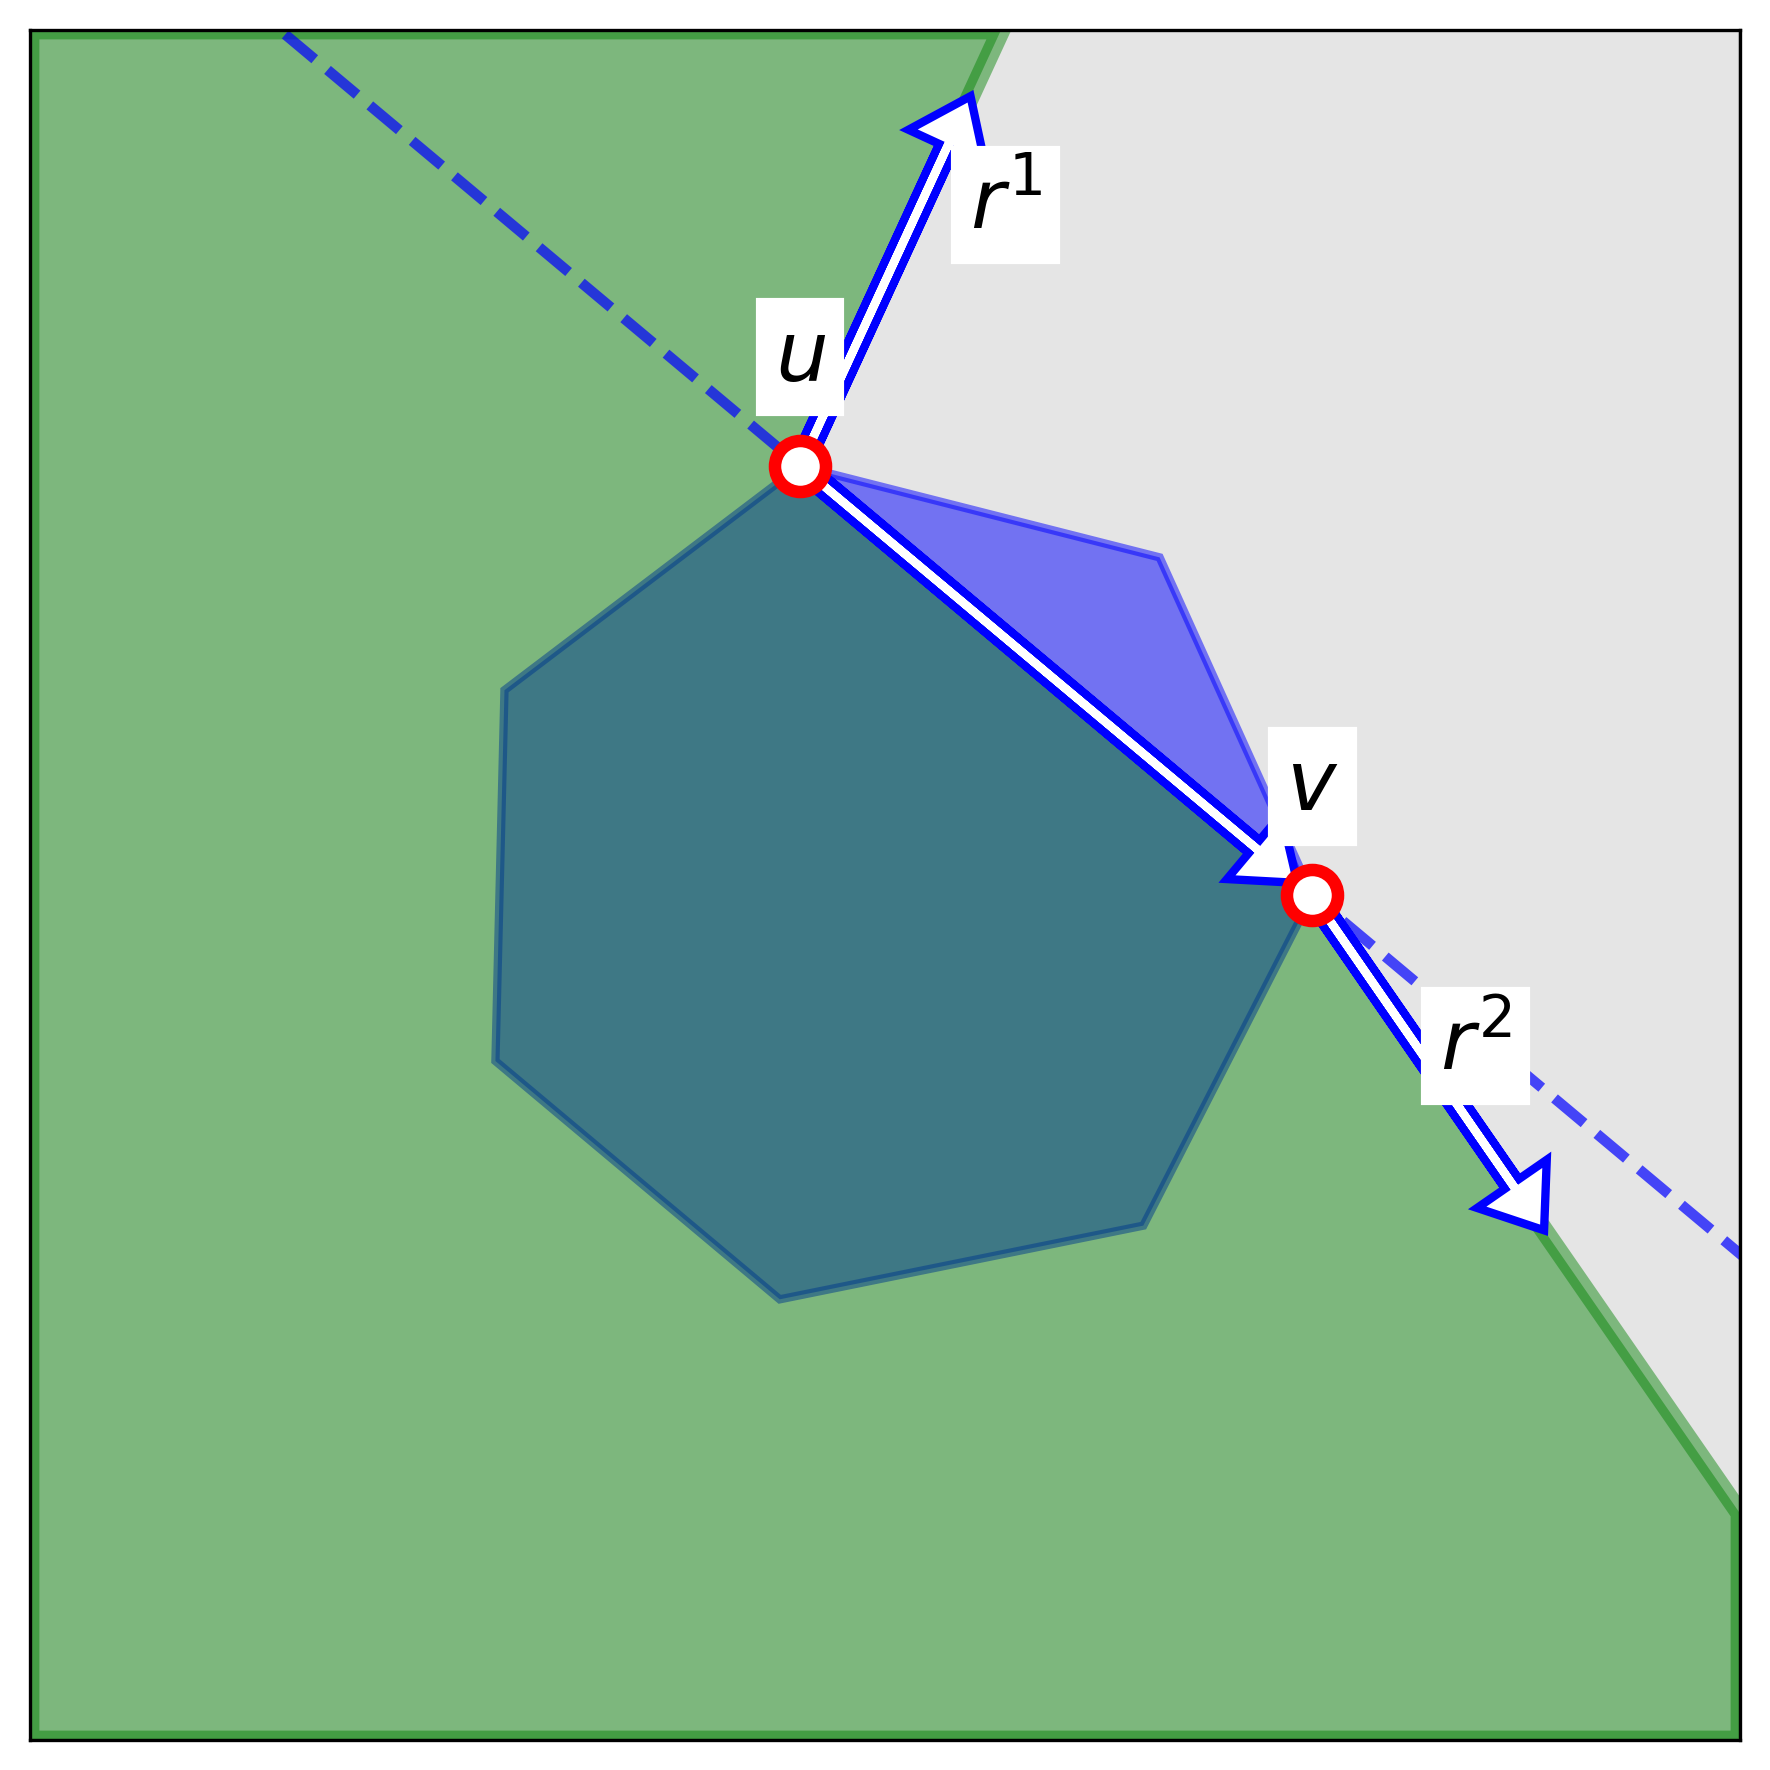
\includegraphics[width=\textwidth]{binary_search_cases-4.png}
		\caption{\(r^1\) interno,~\(r^2\) externo.}
	\end{subfigure}
	\caption{Casos para verificação de pertinência à região de uma aresta fictícia.}
	\label{fig:binary_search_cases}
\end{figure}

Com essa ferramenta, aplica-se busca binária sobre os vértices de~\(P_i\): mantém-se um intervalo~\([l, r]\) com~\(l = 1\) e~\(r = |P_i| + 1\), e a cada passo verifica-se se~\(p\) está entre~\(v^l\) e~\(v^{mid}\). Quando~\(l + 1 = r\), sabe-se que~\(p\) está na região de~\(v^l\) ou de~\(\overline{v^l v^r}\), e basta checar qual dos dois casos se aplica, retornando a região de atravessar se nenhum deles pertencer a~\(T_i\). O custo total é~\(O(\log|P_i|)\), implementado no Algoritmo~\algref{alg:locate_point}.

\begin{algorithm}[h!]
\alglabel{alg:locate_point}
\caption{Localiza Ponto}
\Input{\(p\),~\(P_i\),~\(T_i\),~\(S_i\)}
\Output{Região de~\(S_i\) que contém~\(p\).}
\vspace{0.3em}\hrule\vspace{0.3em}
\Function{VerificaAresta\((u, v, p, S_i)\)}{
	\(r^1 \leftarrow\) primeiro raio de~\(u\) em~\(S_i\) \\
	\(r^2 \leftarrow\) primeiro raio de~\(v\) em~\(S_i\) \\
	\(c_1 \leftarrow r^1 \times (p - u) \ge 0\) \\
	\(c_2 \leftarrow r^2 \times (p - v) \le 0\) \\
	\(c_3 \leftarrow (v - u) \times (p - u) \le 0\) \\
	\If{\((v - u) \times r^1 < 0\)}{
		\If{\((v - u) \times r^2 < 0\)}{ \Return{}~\(c_1 \land c_2 \land c_3\) }
		\Else{ \Return{}~\((c_1 \land c_3) \lor (c_2 \land \lnot c_3)\) }
	}
	\Else{
		\If{\((v - u) \times r^2 < 0\)}{ \Return{}~\((c_1 \land \lnot c_3) \lor (c_2 \land c_3)\) }
		\Else{ \Return{}~\(c_1 \lor c_2 \lor c_3\) }
	}
}
\Function{LocalizaPonto\((p, P_i, T_i, S_i)\)}{
	\(l \leftarrow 1\), \quad~\(r \leftarrow |P_i| + 1\) \\
	\While{\(l + 1 \ne r\)}{
		\(mid \leftarrow \lfloor(l + r) / 2\rfloor\) \\
		\If{VerificaAresta\((v^l, v^{mid}, p, S_i)\)}{~\(r \leftarrow mid\) }
		\Else{~\(l \leftarrow mid\) }
	}
	\If{\(v^l \in T_i\) e~\(p\) está na região de~\(v^l\)}{ \Return{} região de~\(v^l\) }
	\ElseIf{\(\overline{v^l v^r} \in T_i\)}{ \Return{} região de~\(\overline{v^l v^r}\) }
	\Else{ \Return{} região de atravessar }
}
\end{algorithm}

\subsubsection{Consulta ao Caminho}
\label{sec:query}

Com \texttt{LocalizaPonto} definido, pode-se implementar \texttt{ConsultaÚltimoPasso} e \texttt{ConsultaCaminho}. Ambas operam recursivamente sobre os mesmos três casos: se~\(p\) está em uma região de vértice~\(v\), o~\(i\)-path até~\(p\) é o~\((i-1)\)-path até~\(v\) seguido de~\(\overline{vp}\); se está em uma região de aresta~\(e = \overline{uv}\), reflete-se~\(p\) em relação à reta que contém~\(e\) obtendo~\(p'\), calcula-se o~\((i-1)\)-path até~\(p'\) e toma-se a interseção do último segmento com~\(e\) como ponto de contato; se está na região de atravessar, o~\(i\)-path até~\(p\) coincide com o~\((i-1)\)-path até~\(p\).

A distinção entre as duas funções é que \texttt{ConsultaÚltimoPasso} retorna apenas o ponto que precede~\(p\) no~\(i\)-path, sem reconstruir o caminho completo. Isso permite uma otimização importante: no caso de região de vértice,~\(v\) é imediatamente o ponto predecessor, sem necessidade de recursão adicional. Essa função é usada pelos Algoritmos~\algref{alg:first_contact_region} e~\algref{alg:last_step_map}, que precisam apenas do último passo e não do caminho completo. Ambas as funções estão implementadas no Algoritmo~\algref{alg:query}.

\begin{algorithm}[h!]
\alglabel{alg:query}
\caption{Consulta Caminho e Último Passo}
\Input{\(p, i, s, (P_1, \dots, P_i), (T_1, \dots, T_i), (S_1, \dots, S_i)\)}
\Output{\(i\)-path até~\(p\) (ou apenas o ponto que o precede).}
\vspace{0.3em}\hrule\vspace{0.3em}
\Function{ConsultaÚltimoPasso\((p, i, \dots)\)}{
	\If{\(i = 0\)}{ \Return{}~\(s\) }
	\(R \leftarrow \text{LocalizaPonto}(p, P_i, T_i, S_i)\) \\
	\If{\(R\) é região de vértice~\(v\)}{ \Return{}~\(v\) }
	\ElseIf{\(R\) é região de aresta~\(e = \overline{uv}\)}{
		\(p' \leftarrow\) reflexão de~\(p\) em relação à reta de~\(e\) \\
		\(q' \leftarrow \text{ConsultaÚltimoPasso}(p', i-1, \dots)\) \\
		\Return{} interseção de~\(\overline{q'p'}\) com~\(e\)
	}
	\Else{ \Return{}~\(\text{ConsultaÚltimoPasso}(p, i-1, \dots)\) }
}
\Function{ConsultaCaminho\((p, i, \dots)\)}{
	\If{\(i = 0\)}{ \Return{}~\([s]\) }
	\(R \leftarrow \text{LocalizaPonto}(p, P_i, T_i, S_i)\) \\
	\If{\(R\) é região de vértice~\(v\)}{
		\Return{}~\(\text{ConsultaCaminho}(v, i-1, \dots) \oplus [v]\)
	}
	\ElseIf{\(R\) é região de aresta~\(e = \overline{uv}\)}{
		\(p' \leftarrow\) reflexão de~\(p\) em relação à reta de~\(e\) \\
		\(\mathbb{P} \leftarrow \text{ConsultaCaminho}(p', i-1, \dots)\) \\
		\(q \leftarrow\) interseção de~\(\overline{(\text{último de } \mathbb{P})\,p'}\) com~\(e\) \\
		\Return{}~\(\mathbb{P} \oplus [q]\)
	}
	\Else{ \Return{}~\(\text{ConsultaCaminho}(p, i-1, \dots)\) }
}
\end{algorithm}

\subsubsection{Implementação Completa}

O algoritmo completo para o TPP Convexo itera sobre os polígonos calculando~\(T_i\) e~\(S_i\) em ordem, e ao final consulta o~\(k\)-path até~\(t\), conforme o Algoritmo~\algref{alg:tpp_complete}.

\begin{algorithm}[h!]
\alglabel{alg:tpp_complete}
\caption{TPP Convexo}
\Input{Pontos~\(s\) e~\(t\), polígonos convexos disjuntos~\((P_1, \dots, P_k)\)}
\Output{\(k\)-path até~\(t\).}
\vspace{0.3em}\hrule\vspace{0.3em}
\Function{TPPConvexo\((s, t, P_1, \dots, P_k)\)}{
	\For{\(i \leftarrow 1\) até~\(k\)}{
		\(T_i \leftarrow \text{RegiãoDePrimeiroContato}(i, s, \dots)\) \\
		\(S_i \leftarrow \text{MapaDeÚltimoPasso}(i, s, \dots)\)
	}
	\Return{}~\(\text{ConsultaCaminho}(t, k, s, \dots)\)
}
\end{algorithm}

\subsection{Análise de Complexidade}

Adota-se a seguinte notação: seja~\(|P_i|\) o número de vértices do polígono~\(P_i\), seja~\(k\) o número de polígonos e~\(n = \sum_{i=1}^{k} |P_i|\) o número total de vértices.

Analisa-se a complexidade de cada componente do algoritmo, de baixo para cima.

\begin{description}

\item[\texttt{LocalizaPonto}:] A busca binária realiza~\(O(\log|P_i|)\) chamadas a \texttt{VerificaAresta}, cada uma em tempo~\(O(1)\). Portanto, \texttt{LocalizaPonto} tem complexidade~\(O(\log|P_i|)\).

\item[\texttt{ConsultaÚltimoPasso}:] No pior caso, o ponto consultado está na região de atravessar de todos os polígonos~\(P_i, P_{i-1}, \dots, P_1\), resultando em~\(i\) chamadas a \texttt{LocalizaPonto}. A complexidade é portanto:
\[
	O\!\left(\sum_{j=1}^{i} \log|P_j|\right).
\]

\item[\texttt{RegiãoDePrimeiroContato} e \texttt{MapaDeÚltimoPasso}:] Ambos iteram sobre os~\(|P_i|\) vértices de~\(P_i\), realizando uma chamada a \texttt{ConsultaÚltimoPasso} por vértice. A complexidade de cada um é:
\[
	O\!\left(|P_i| \sum_{j=1}^{i} \log|P_j|\right).
\]

\item[Algoritmo completo:] O algoritmo calcula~\(T_i\) e~\(S_i\) para~\(i = 1, \dots, k\) e ao final consulta o~\(k\)-path até~\(t\). O custo total é:
\begin{align*}
	O\!\left(\sum_{i=1}^{k} |P_i| \sum_{j=1}^{i} \log|P_j|\right)
	&= O\!\left(\sum_{i=1}^{k} |P_i| \sum_{j=1}^{k} \log|P_j|\right) \\
	&= O\!\left(n \sum_{j=1}^{k} \log|P_j|\right).
\end{align*}
A soma~\(\sum_{j=1}^{k} \log|P_j|\) é maximizada quando os polígonos têm o mesmo número de vértices, isto é,~\(|P_j| = n/k\) para todo~\(j\), o que dá~\(\sum_{j=1}^{k} \log(n/k) = k\log(n/k)\). Portanto, a complexidade total do algoritmo é:
\[
	O\!\left(nk\log(n/k)\right),
\]
que coincide com a complexidade apresentada por Dror et al.~\cite{tpp-dror-2003}.

\end{description}

\subsection{Experimentos Computacionais}

Os experimentos foram conduzidos em um MacBook Pro com chip Apple M4 Pro (12 núcleos, sendo 8 de desempenho e 4 de eficiência) e 24 GB de memória. O código foi compilado com GCC 15.2.0 usando C++23 e otimização~\texttt{-O3}. Para acelerar a execução dos testes, utilizou-se paralelismo via OpenMP, porém os tempos registrados correspondem à execução sequencial de cada instância individualmente.

O objetivo dos experimentos é verificar que o comportamento assintótico do algoritmo está de acordo com a complexidade~\(O(nk\log(n/k))\) prevista pela análise teórica. Utilizaram-se instâncias sintéticas com~\(k\) polígonos regulares de~\(m\) vértices cada, dispostos de forma que todo ponto de~\(P_i\) esteja na região de atravessar de~\(P_j\) para todo~\(j < i\), representando o pior caso do algoritmo. Nessa configuração,~\(n = mk\) e a complexidade teórica é~\(O(m\log(m) \cdot k^2)\).

Realizaram-se dois experimentos. No primeiro, fixou-se~\(m \in \{5, 50\}\) e variou-se~\(k\) de~\(1\) até~\(3000\), com~\(300\) medições uniformemente espaçadas. Para cada valor de~\(m\), ajustou-se um modelo da forma~\(c_0 + c_1 k + c_2 k^2\) aos dados de tempo de execução por mínimos quadrados; a curva ajustada é exibida junto com os dados na Figura~\ref{fig:plt_vs_k}. Os resultados mostram que o tempo de execução cresce de forma quadrática em~\(k\), conforme previsto.

\begin{figure}[!ht]
	\centering
	\begin{subfigure}[b]{0.45\textwidth}
		\centering
		
\includegraphics[width=\textwidth]{plt_vs_k_m_5.png}
		\caption{Resultados para~\(m = 5\).}
	\end{subfigure}
	\hspace{10pt}
	\begin{subfigure}[b]{0.45\textwidth}
		\centering
		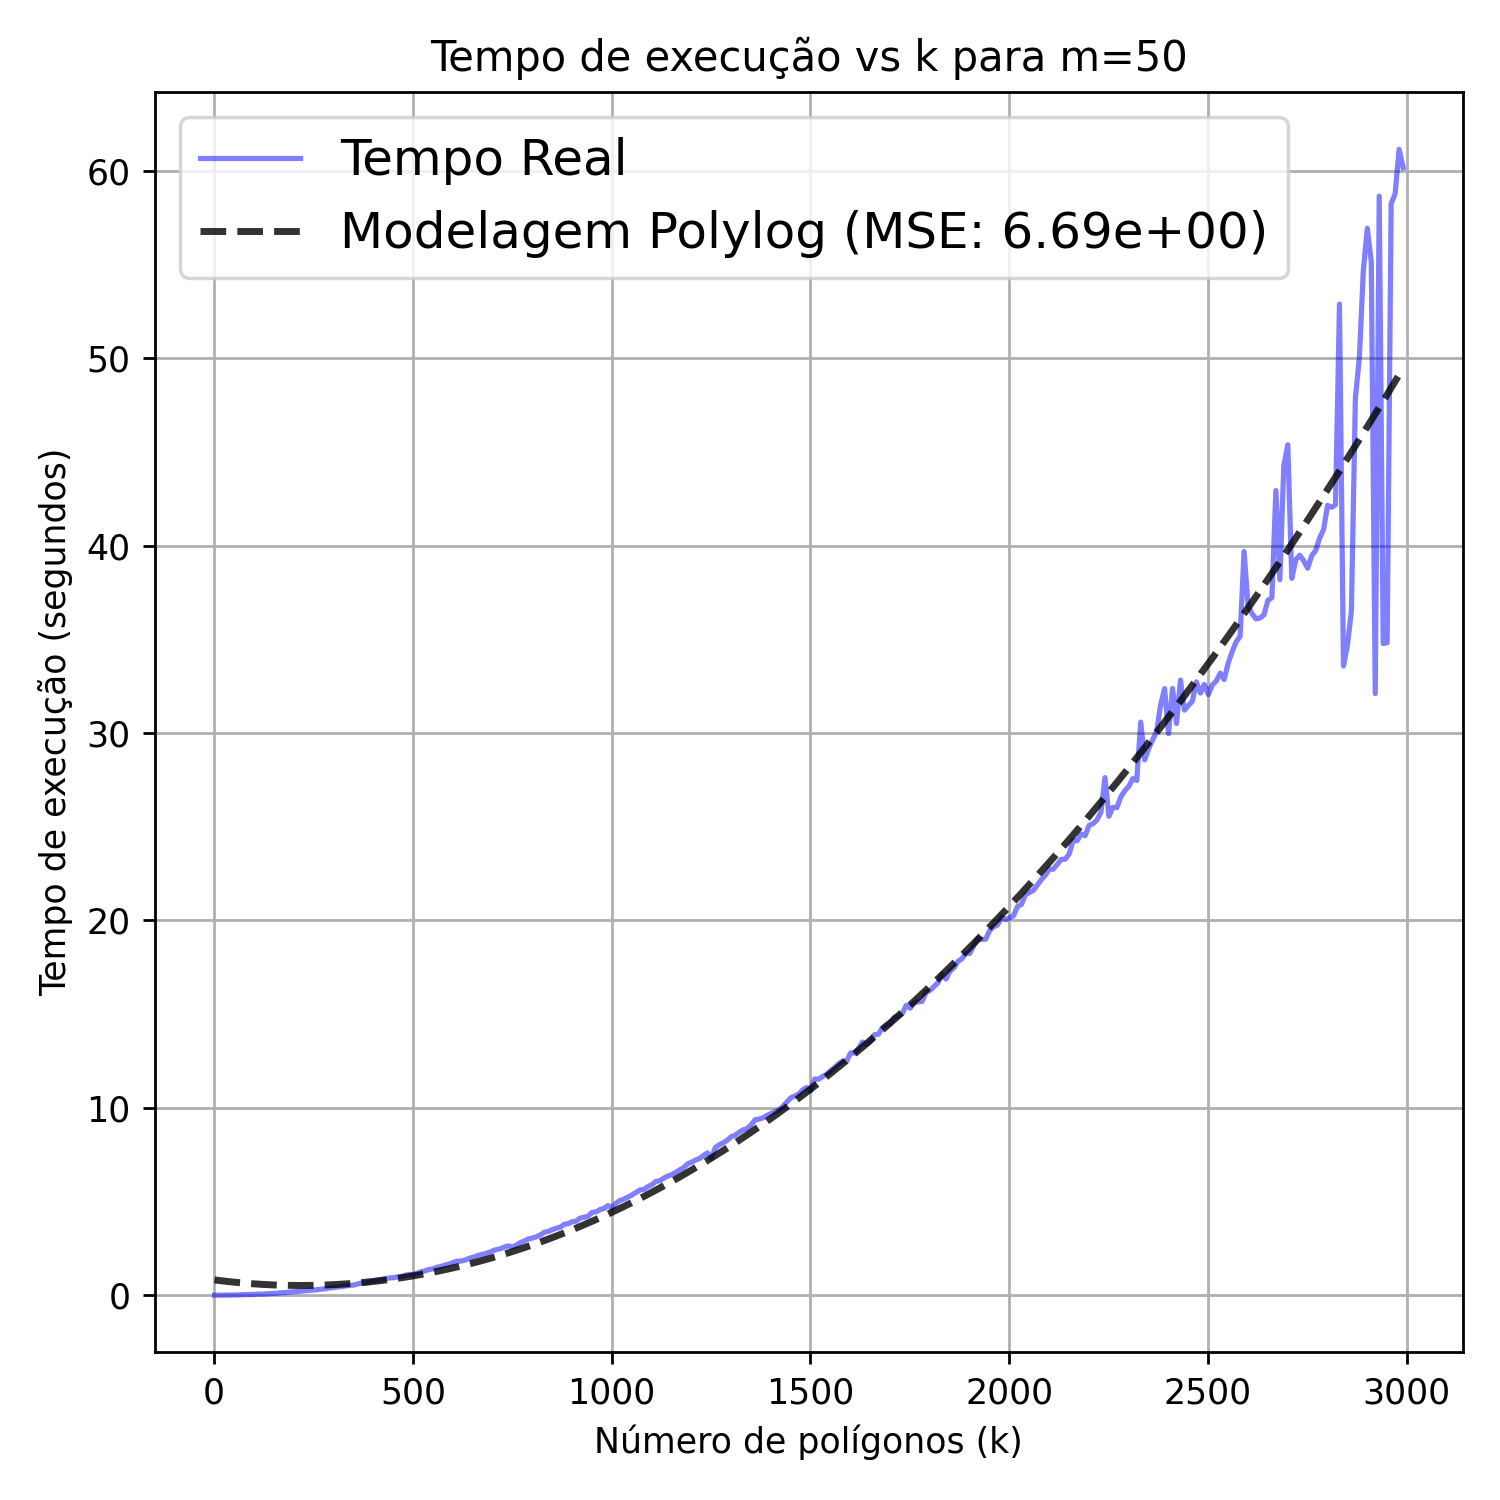
\includegraphics[width=\textwidth]{plt_vs_k_m_50.png}
		\caption{Resultados para~\(m = 50\).}
	\end{subfigure}
	\caption{Tempo de execução em função de~\(k\) para dois valores de~\(m\). A curva tracejada corresponde ao modelo ajustado por mínimos quadrados.}
	\label{fig:plt_vs_k}
\end{figure}

\begin{figure}[!ht]
	\centering
	\begin{subfigure}[b]{0.45\textwidth}
		\centering
		
\includegraphics[width=\textwidth]{plt_vs_m_k_5.png}
		\caption{Resultados para~\(k = 5\).}
	\end{subfigure}
	\hspace{10pt}
	\begin{subfigure}[b]{0.45\textwidth}
		\centering
		
\includegraphics[width=\textwidth]{plt_vs_m_k_20.png}
		\caption{Resultados para~\(k = 20\).}
	\end{subfigure}
	\caption{Tempo de execução em função de~\(m\) para dois valores de~\(k\). A curva tracejada corresponde ao modelo ajustado por mínimos quadrados.}
	\label{fig:plt_vs_m}
\end{figure}

No segundo experimento, fixou-se~\(k \in \{5, 20\}\) e variou-se~\(m\) de~\(3\) até~\(40000\), com~\(400\) medições uniformemente espaçadas. Para cada valor de~\(k\), ajustou-se um modelo da forma~\(c_0 + c_1(n+k) + c_2 nk + c_3 nk\log(n/k)\) por mínimos quadrados; a curva ajustada é exibida na Figura~\ref{fig:plt_vs_m}. As curvas têm aspecto aproximadamente linear, o que é esperado: o fator~\(\log(m)\) varia apenas de~\(\log(3) \approx 1{,}6\) a~\(\log(40000) \approx 10{,}6\) na faixa considerada, uma variação de apenas~\(6\times\) em uma escala de~\(40000\times\), tornando-o imperceptível visualmente. O ajuste do modelo polilogarítmico confirma, no entanto, que os coeficientes são consistentes com a complexidade teórica.

\section{Ferramenta de Visualização}
\label{sec:visualizer}

Como parte do trabalho desenvolvido neste período, implementou-se uma ferramenta de visualização interativa para o TPP, disponível em \url{https://yushipy.github.io/PersonalPage/Visualizer/index.html}. A ferramenta permite construir instâncias do problema diretamente no navegador, definir os pontos~\(s\) e~\(t\), editar polígonos e acionar o algoritmo para computar o caminho ótimo.

Para instâncias com polígonos convexos, é possível exibir o mapa de último passo do polígono selecionado, colorindo as regiões de vértice em vermelho, as regiões de aresta em verde e a região de atravessar em ciano. A Figura~\ref{fig:visualizer} apresenta uma captura de tela da ferramenta com uma instância de exemplo.

\begin{figure}[!ht]
	\centering
	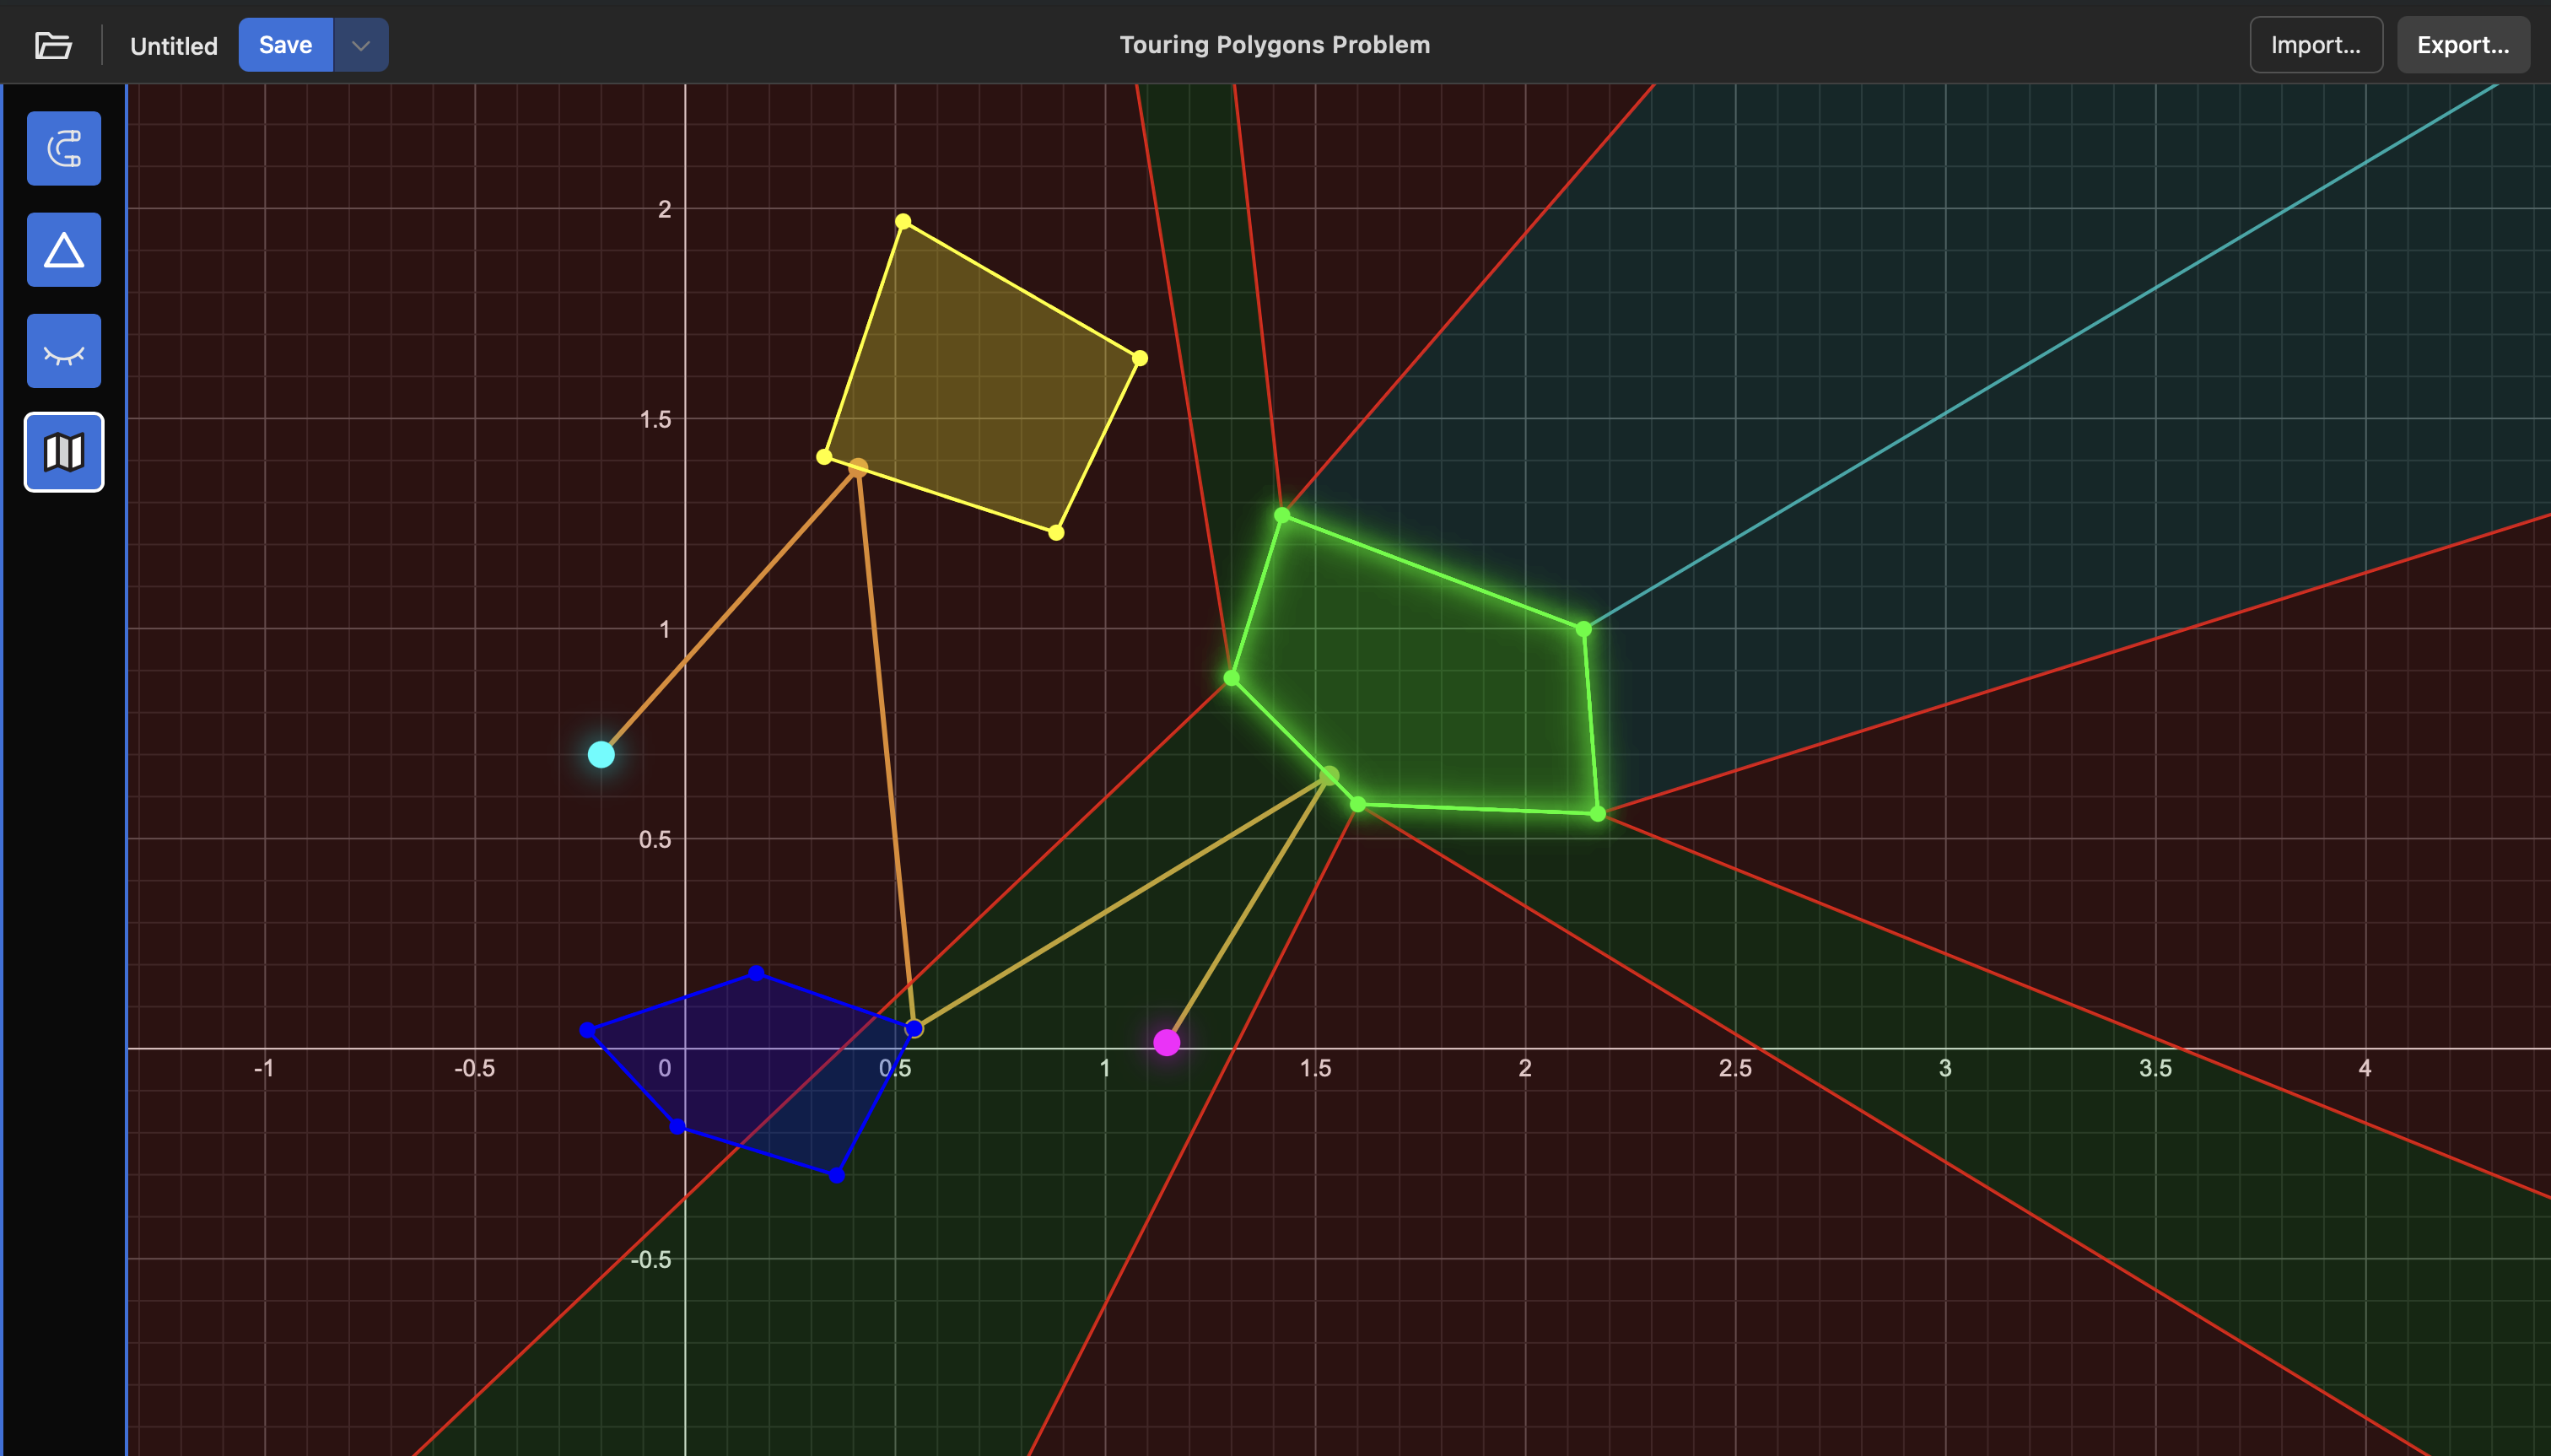
\includegraphics[width=0.85\textwidth]{visualizer.png}
	\caption{Ferramenta de visualização interativa do TPP, exibindo uma instância com três polígonos convexos, o caminho ótimo encontrado e o mapa de último passo \(S_3\) do terceiro polígono.}
	\label{fig:visualizer}
\end{figure}

A ferramenta foi projetada para acompanhar o desenvolvimento do projeto: à medida que o suporte ao caso não convexo for implementado nas etapas seguintes, a visualização será estendida para cobrir essas instâncias. No momento da escrita deste relatório, instâncias com polígonos não convexos desativam automaticamente a exibição dos mapas de último passo. Uma documentação detalhada das funcionalidades está disponível em \url{https://yushipy.github.io/PersonalPage/Visualizer/tpp-info.html#toolbar}.

\section{Plano de Atividades para o Próximo Período}
\label{sec:proximos_passos}

O próximo período será dedicado ao TPP não convexo com ordem fixa, que é NP-difícil~\cite{tpp-dror-2003}. A abordagem planejada consiste em decompor cada polígono não convexo em peças convexas, usando o algoritmo de Greene~\cite{cpd-greene-1983} disponível na biblioteca CGAL~\cite{cgal}, e aplicar o algoritmo desenvolvido neste período a cada combinação possível de peças, explorando técnicas de Branch and Bound para tornar essa busca tratável na prática.

As atividades previstas são as seguintes:

\begin{enumerate}
	\item Integrar a decomposição convexa de polígonos não convexos via algoritmo de Greene~\cite{cpd-greene-1983}, disponível na biblioteca CGAL~\cite{cgal}.

	\item Formular e implementar o algoritmo de Branch and Bound para o TPP não convexo. Cada nó da árvore de busca atribui uma peça convexa a cada polígono; o lower bound é obtido resolvendo o TPP convexo com os convex hulls dos polígonos ainda não atribuídos.

	\item Calcular uma solução inicial de boa qualidade para inicializar o Branch and Bound, reduzindo o espaço de busca explorado.

	\item Implementar um baseline via programação inteira mista com o solver Gurobi~\cite{gurobi} para verificar a corretude e comparar o desempenho do Branch and Bound.

	\item Estender a ferramenta de visualização para suportar instâncias com polígonos não convexos.

	\item Realizar experimentos computacionais para avaliar o desempenho do Branch and Bound em instâncias de diferentes tamanhos e características.
\end{enumerate}

Paralelamente, será submetida à FAPESP uma solicitação de bolsa BEPE para dar continuidade ao projeto em estágio de pesquisa no exterior. A proposta prevê uma visita de quatro meses à Université Laval, no Canadá, sob supervisão do Prof.\ Leandro Callegari Coelho, cujo grupo de pesquisa possui ampla experiência em métodos exatos para problemas de roteamento de veículos. O foco da etapa no exterior será o TPP sem ordem fixa de visita, variante NP-difícil que generaliza o TPP não convexo e equivale ao problema de roteamento de veículo único com vizinhanças poligonais não convexas.

\bibliographystyle{plain}
\bibliography{referencias}

\end{document}
